% Options for packages loaded elsewhere
% Options for packages loaded elsewhere
\PassOptionsToPackage{unicode}{hyperref}
\PassOptionsToPackage{hyphens}{url}
%
\documentclass[
  ignorenonframetext,
  aspectratio=169,
]{beamer}
\newif\ifbibliography
\usepackage{pgfpages}
\setbeamertemplate{caption}[numbered]
\setbeamertemplate{caption label separator}{: }
\setbeamercolor{caption name}{fg=normal text.fg}
\beamertemplatenavigationsymbolsempty
% remove section numbering
\setbeamertemplate{part page}{
  \centering
  \begin{beamercolorbox}[sep=16pt,center]{part title}
    \usebeamerfont{part title}\insertpart\par
  \end{beamercolorbox}
}
\setbeamertemplate{section page}{
  \centering
  \begin{beamercolorbox}[sep=12pt,center]{section title}
    \usebeamerfont{section title}\insertsection\par
  \end{beamercolorbox}
}
\setbeamertemplate{subsection page}{
  \centering
  \begin{beamercolorbox}[sep=8pt,center]{subsection title}
    \usebeamerfont{subsection title}\insertsubsection\par
  \end{beamercolorbox}
}
% Prevent slide breaks in the middle of a paragraph
\widowpenalties 1 10000
\raggedbottom
\AtBeginPart{
  \frame{\partpage}
}
\AtBeginSection{
  \ifbibliography
  \else
    \frame{\sectionpage}
  \fi
}
\AtBeginSubsection{
  \frame{\subsectionpage}
}
\usepackage{iftex}
\ifPDFTeX
  \usepackage[T1]{fontenc}
  \usepackage[utf8]{inputenc}
  \usepackage{textcomp} % provide euro and other symbols
\else % if luatex or xetex
  \usepackage{unicode-math} % this also loads fontspec
  \defaultfontfeatures{Scale=MatchLowercase}
  \defaultfontfeatures[\rmfamily]{Ligatures=TeX,Scale=1}
\fi
\usepackage{lmodern}

\usetheme[]{Boadilla}
\usecolortheme[]{default}
\usefonttheme[]{professionalfonts}
\ifPDFTeX\else
  % xetex/luatex font selection
\fi
% Use upquote if available, for straight quotes in verbatim environments
\IfFileExists{upquote.sty}{\usepackage{upquote}}{}
\IfFileExists{microtype.sty}{% use microtype if available
  \usepackage[]{microtype}
  \UseMicrotypeSet[protrusion]{basicmath} % disable protrusion for tt fonts
}{}
\makeatletter
\@ifundefined{KOMAClassName}{% if non-KOMA class
  \IfFileExists{parskip.sty}{%
    \usepackage{parskip}
  }{% else
    \setlength{\parindent}{0pt}
    \setlength{\parskip}{6pt plus 2pt minus 1pt}}
}{% if KOMA class
  \KOMAoptions{parskip=half}}
\makeatother

\usepackage{color}
\usepackage{fancyvrb}
\newcommand{\VerbBar}{|}
\newcommand{\VERB}{\Verb[commandchars=\\\{\}]}
\DefineVerbatimEnvironment{Highlighting}{Verbatim}{commandchars=\\\{\}}
% Add ',fontsize=\small' for more characters per line
\usepackage{framed}
\definecolor{shadecolor}{RGB}{241,243,245}
\newenvironment{Shaded}{\begin{snugshade}}{\end{snugshade}}
\newcommand{\AlertTok}[1]{\textcolor[rgb]{0.68,0.00,0.00}{#1}}
\newcommand{\AnnotationTok}[1]{\textcolor[rgb]{0.37,0.37,0.37}{#1}}
\newcommand{\AttributeTok}[1]{\textcolor[rgb]{0.40,0.45,0.13}{#1}}
\newcommand{\BaseNTok}[1]{\textcolor[rgb]{0.68,0.00,0.00}{#1}}
\newcommand{\BuiltInTok}[1]{\textcolor[rgb]{0.00,0.23,0.31}{#1}}
\newcommand{\CharTok}[1]{\textcolor[rgb]{0.13,0.47,0.30}{#1}}
\newcommand{\CommentTok}[1]{\textcolor[rgb]{0.37,0.37,0.37}{#1}}
\newcommand{\CommentVarTok}[1]{\textcolor[rgb]{0.37,0.37,0.37}{\textit{#1}}}
\newcommand{\ConstantTok}[1]{\textcolor[rgb]{0.56,0.35,0.01}{#1}}
\newcommand{\ControlFlowTok}[1]{\textcolor[rgb]{0.00,0.23,0.31}{\textbf{#1}}}
\newcommand{\DataTypeTok}[1]{\textcolor[rgb]{0.68,0.00,0.00}{#1}}
\newcommand{\DecValTok}[1]{\textcolor[rgb]{0.68,0.00,0.00}{#1}}
\newcommand{\DocumentationTok}[1]{\textcolor[rgb]{0.37,0.37,0.37}{\textit{#1}}}
\newcommand{\ErrorTok}[1]{\textcolor[rgb]{0.68,0.00,0.00}{#1}}
\newcommand{\ExtensionTok}[1]{\textcolor[rgb]{0.00,0.23,0.31}{#1}}
\newcommand{\FloatTok}[1]{\textcolor[rgb]{0.68,0.00,0.00}{#1}}
\newcommand{\FunctionTok}[1]{\textcolor[rgb]{0.28,0.35,0.67}{#1}}
\newcommand{\ImportTok}[1]{\textcolor[rgb]{0.00,0.46,0.62}{#1}}
\newcommand{\InformationTok}[1]{\textcolor[rgb]{0.37,0.37,0.37}{#1}}
\newcommand{\KeywordTok}[1]{\textcolor[rgb]{0.00,0.23,0.31}{\textbf{#1}}}
\newcommand{\NormalTok}[1]{\textcolor[rgb]{0.00,0.23,0.31}{#1}}
\newcommand{\OperatorTok}[1]{\textcolor[rgb]{0.37,0.37,0.37}{#1}}
\newcommand{\OtherTok}[1]{\textcolor[rgb]{0.00,0.23,0.31}{#1}}
\newcommand{\PreprocessorTok}[1]{\textcolor[rgb]{0.68,0.00,0.00}{#1}}
\newcommand{\RegionMarkerTok}[1]{\textcolor[rgb]{0.00,0.23,0.31}{#1}}
\newcommand{\SpecialCharTok}[1]{\textcolor[rgb]{0.37,0.37,0.37}{#1}}
\newcommand{\SpecialStringTok}[1]{\textcolor[rgb]{0.13,0.47,0.30}{#1}}
\newcommand{\StringTok}[1]{\textcolor[rgb]{0.13,0.47,0.30}{#1}}
\newcommand{\VariableTok}[1]{\textcolor[rgb]{0.07,0.07,0.07}{#1}}
\newcommand{\VerbatimStringTok}[1]{\textcolor[rgb]{0.13,0.47,0.30}{#1}}
\newcommand{\WarningTok}[1]{\textcolor[rgb]{0.37,0.37,0.37}{\textit{#1}}}

\usepackage{longtable,booktabs,array}
\newcounter{none} % for unnumbered tables
\usepackage{calc} % for calculating minipage widths
\usepackage{caption}
% Make caption package work with longtable
\makeatletter
\def\fnum@table{\tablename~\thetable}
\makeatother
\usepackage{graphicx}
\makeatletter
\newsavebox\pandoc@box
\newcommand*\pandocbounded[1]{% scales image to fit in text height/width
  \sbox\pandoc@box{#1}%
  \Gscale@div\@tempa{\textheight}{\dimexpr\ht\pandoc@box+\dp\pandoc@box\relax}%
  \Gscale@div\@tempb{\linewidth}{\wd\pandoc@box}%
  \ifdim\@tempb\p@<\@tempa\p@\let\@tempa\@tempb\fi% select the smaller of both
  \ifdim\@tempa\p@<\p@\scalebox{\@tempa}{\usebox\pandoc@box}%
  \else\usebox{\pandoc@box}%
  \fi%
}
% Set default figure placement to htbp
\def\fps@figure{htbp}
\makeatother





\setlength{\emergencystretch}{3em} % prevent overfull lines

\providecommand{\tightlist}{%
  \setlength{\itemsep}{0pt}\setlength{\parskip}{0pt}}



 


\makeatletter
\@ifpackageloaded{tcolorbox}{}{\usepackage[skins,breakable]{tcolorbox}}
\@ifpackageloaded{fontawesome5}{}{\usepackage{fontawesome5}}
\definecolor{quarto-callout-color}{HTML}{909090}
\definecolor{quarto-callout-note-color}{HTML}{0758E5}
\definecolor{quarto-callout-important-color}{HTML}{CC1914}
\definecolor{quarto-callout-warning-color}{HTML}{EB9113}
\definecolor{quarto-callout-tip-color}{HTML}{00A047}
\definecolor{quarto-callout-caution-color}{HTML}{FC5300}
\definecolor{quarto-callout-color-frame}{HTML}{acacac}
\definecolor{quarto-callout-note-color-frame}{HTML}{4582ec}
\definecolor{quarto-callout-important-color-frame}{HTML}{d9534f}
\definecolor{quarto-callout-warning-color-frame}{HTML}{f0ad4e}
\definecolor{quarto-callout-tip-color-frame}{HTML}{02b875}
\definecolor{quarto-callout-caution-color-frame}{HTML}{fd7e14}
\makeatother
\makeatletter
\@ifpackageloaded{caption}{}{\usepackage{caption}}
\AtBeginDocument{%
\ifdefined\contentsname
  \renewcommand*\contentsname{Table of contents}
\else
  \newcommand\contentsname{Table of contents}
\fi
\ifdefined\listfigurename
  \renewcommand*\listfigurename{List of Figures}
\else
  \newcommand\listfigurename{List of Figures}
\fi
\ifdefined\listtablename
  \renewcommand*\listtablename{List of Tables}
\else
  \newcommand\listtablename{List of Tables}
\fi
\ifdefined\figurename
  \renewcommand*\figurename{Figure}
\else
  \newcommand\figurename{Figure}
\fi
\ifdefined\tablename
  \renewcommand*\tablename{Table}
\else
  \newcommand\tablename{Table}
\fi
}
\@ifpackageloaded{float}{}{\usepackage{float}}
\floatstyle{ruled}
\@ifundefined{c@chapter}{\newfloat{codelisting}{h}{lop}}{\newfloat{codelisting}{h}{lop}[chapter]}
\floatname{codelisting}{Listing}
\newcommand*\listoflistings{\listof{codelisting}{List of Listings}}
\makeatother
\makeatletter
\makeatother
\makeatletter
\@ifpackageloaded{caption}{}{\usepackage{caption}}
\@ifpackageloaded{subcaption}{}{\usepackage{subcaption}}
\makeatother

\usepackage{bookmark}
\IfFileExists{xurl.sty}{\usepackage{xurl}}{} % add URL line breaks if available
\urlstyle{same}
\hypersetup{
  pdftitle={02\_Introduction\_to\_Data\_Science\_Slides},
  hidelinks,
  pdfcreator={LaTeX via pandoc}}


\title{\texorpdfstring{02\_Introduction\_to\_Data\_Science\_Slides}{02\_Introduction\_to\_Data\_Science\_Slides}}
\author{}
\date{}

\begin{document}
\frame{\titlepage}


\subsection{Part I --- From Insurance to Data
Science}\label{part-i-from-insurance-to-data-science}

\begin{frame}{Why Data Science in Insurance?}
\protect\phantomsection\label{why-data-science-in-insurance}
Insurance is fundamentally concerned with making decisions under
uncertainty.

As actuaries, we use probability, statistics, and insurance principles
to assess risk. In practice, these decisions also require reliable data
and systematic methods for analysing it.

For example, a motor insurer may want to determine whether claim
frequency differs according to:

\begin{itemize}
\tightlist
\item
  age;
\item
  geographical area;
\item
  vehicle characteristics; or
\item
  other characteristics of policyholders.
\end{itemize}

Data science provides a framework for investigating such questions.
\end{frame}

\begin{frame}{Data-Driven Insurance Decisions}
\protect\phantomsection\label{data-driven-insurance-decisions}
An insurance decision is \textbf{data-driven} when relevant data are
used systematically to support the decision.

Data do not replace actuarial judgement. They provide evidence that can
be combined with:

\begin{itemize}
\tightlist
\item
  statistical methods;
\item
  insurance knowledge; and
\item
  professional judgement.
\end{itemize}

Insurers use data to:

\begin{itemize}
\tightlist
\item
  assess and classify risks during underwriting;
\item
  estimate claim frequency and claim severity;
\item
  determine appropriate premiums;
\item
  monitor claims and identify unusual patterns;
\item
  evaluate portfolio experience; and
\item
  support risk-management decisions.
\end{itemize}
\end{frame}

\begin{frame}{From Data to Decision}
\protect\phantomsection\label{from-data-to-decision}
Consider a motor insurance portfolio.

Suppose an insurer observes that policyholders in different age groups
have different claim frequencies.

The insurer needs to determine whether this difference is supported by
sufficient data and whether age should be considered when assessing
risk.

\[
\text{Insurance problem}
\rightarrow
\text{Data}
\rightarrow
\text{Analysis}
\rightarrow
\text{Evidence}
\rightarrow
\text{Decision}.
\]

The purpose of data science is therefore to transform data into useful
information and evidence for decision-making.
\end{frame}

\begin{frame}{Data Do Not Speak for Themselves}
\protect\phantomsection\label{data-do-not-speak-for-themselves}
Observed patterns in insurance data must be interpreted in context.

A difference between two groups does not necessarily imply that the
corresponding risk factor causes the difference.

When interpreting an observed pattern, we should consider:

\begin{itemize}
\tightlist
\item
  data quality;
\item
  exposure;
\item
  other relevant risk factors; and
\item
  the method of analysis.
\end{itemize}

\begin{tcolorbox}[enhanced jigsaw, arc=.35mm, bottomrule=.15mm, bottomtitle=1mm, breakable, colback=white, colbacktitle=quarto-callout-note-color!10!white, colframe=quarto-callout-note-color-frame, coltitle=black, left=2mm, leftrule=.75mm, opacityback=0, opacitybacktitle=0.6, rightrule=.15mm, title=\textcolor{quarto-callout-note-color}{\faInfo}\hspace{0.5em}{Key idea}, titlerule=0mm, toprule=.15mm, toptitle=1mm]

\textbf{An observed pattern is evidence, not automatically an
explanation.}

Data science helps us identify and quantify patterns, while actuarial
judgement is needed to interpret those patterns in context.

\end{tcolorbox}
\end{frame}

\begin{frame}{From Risk to Data}
\protect\phantomsection\label{from-risk-to-data}
The concepts of risk introduced in Chapter 1 are theoretical.

In practice, quantities such as probabilities and expected losses must
be estimated from observations.

Suppose an insurer wants to estimate claim frequency from historical
data.

A simple estimate is

\[
\widehat{\lambda}
=
\frac{\text{Number of claims}}
{\text{Exposure}}.
\]

The estimate is obtained from observed insurance experience.
\end{frame}

\begin{frame}{Estimating Claim Severity}
\protect\phantomsection\label{estimating-claim-severity}
Suppose the observed claim amounts are

\[
X_1,\ldots,X_n.
\]

A basic estimate of the average claim amount is

\[
\widehat{\mu}
=
\frac{1}{n}\sum_{i=1}^{n}X_i.
\]

More advanced statistical methods can then be used to investigate how
claim severity varies with different risk characteristics.
\end{frame}

\begin{frame}{From Risk to Risk Assessment}
\protect\phantomsection\label{from-risk-to-risk-assessment}
The transition from actuarial theory to data analysis can be summarised
as

\[
\boxed{
\text{Risk}
\rightarrow
\text{Observable outcomes}
\rightarrow
\text{Data}
\rightarrow
\text{Statistical analysis}
\rightarrow
\text{Risk assessment}
}
\]

Data science provides a systematic framework for the stages involving:

\begin{itemize}
\tightlist
\item
  data collection;
\item
  data preparation;
\item
  exploration;
\item
  analysis and modelling; and
\item
  communication.
\end{itemize}
\end{frame}

\begin{frame}{Exposure Matters}
\protect\phantomsection\label{exposure-matters}
Insurance experience cannot always be compared using raw claim counts.

A portfolio with more policies or a longer observation period will
generally produce more claims simply because there is more opportunity
for claims to occur.

Therefore, insurance experience is often measured relative to an
appropriate measure of \textbf{exposure}.

For example,

\[
\text{Claim frequency}
=
\frac{\text{Number of claims}}
{\text{Exposure}}.
\]

\begin{tcolorbox}[enhanced jigsaw, arc=.35mm, bottomrule=.15mm, bottomtitle=1mm, breakable, colback=white, colbacktitle=quarto-callout-important-color!10!white, colframe=quarto-callout-important-color-frame, coltitle=black, left=2mm, leftrule=.75mm, opacityback=0, opacitybacktitle=0.6, rightrule=.15mm, title=\textcolor{quarto-callout-important-color}{\faExclamation}\hspace{0.5em}{Key idea}, titlerule=0mm, toprule=.15mm, toptitle=1mm]

\textbf{Raw claim counts are not sufficient for comparing insurance
risk.}

The amount of exposure must be considered when measuring claim
experience.

\end{tcolorbox}
\end{frame}

\begin{frame}{Why Data Science Matters to Actuaries}
\protect\phantomsection\label{why-data-science-matters-to-actuaries}
Modern insurance problems often involve large and complex datasets.

An actuary may need to:

\begin{itemize}
\tightlist
\item
  combine information from different sources;
\item
  identify data-quality problems;
\item
  explore relationships between variables;
\item
  develop statistical models; and
\item
  communicate analytical results.
\end{itemize}

However, applying an algorithm to a dataset is not sufficient.

Actuarial knowledge is needed to formulate the problem, select
meaningful variables, recognise appropriate exposure measures, assess
assumptions, and interpret the results.
\end{frame}

\begin{frame}{Data Science and Actuarial Science}
\protect\phantomsection\label{data-science-and-actuarial-science}
{\def\LTcaptype{none} % do not increment counter
\begin{longtable}[]{@{}
  >{\raggedright\arraybackslash}p{(\linewidth - 2\tabcolsep) * \real{0.5000}}
  >{\raggedright\arraybackslash}p{(\linewidth - 2\tabcolsep) * \real{0.5000}}@{}}
\toprule\noalign{}
\begin{minipage}[b]{\linewidth}\raggedright
Data science
\end{minipage} & \begin{minipage}[b]{\linewidth}\raggedright
Actuarial science
\end{minipage} \\
\midrule\noalign{}
\endhead
Collects and prepares data & Understands the insurance problem \\
Explores and visualises data & Interprets risk and uncertainty \\
Develops statistical and predictive models & Assesses actuarial
assumptions and implications \\
Communicates analytical results & Applies professional judgement to
decisions \\
\bottomrule\noalign{}
\end{longtable}
}

The two disciplines are complementary.

\[
\boxed{
\text{Data}
+
\text{Statistical methods}
+
\text{Computing}
+
\text{Actuarial judgement}
}
\]

provides a framework for making better-informed insurance decisions.
\end{frame}

\subsection{Part II --- What Is Data
Science?}\label{part-ii-what-is-data-science}

\begin{frame}{What Is Data Science?}
\protect\phantomsection\label{what-is-data-science}
Data science is concerned with extracting useful information and
knowledge from data to support:

\begin{itemize}
\tightlist
\item
  understanding;
\item
  prediction; and
\item
  decision-making.
\end{itemize}

It combines:

\begin{itemize}
\tightlist
\item
  statistical methods;
\item
  computational tools; and
\item
  knowledge of the subject area in which the data arise.
\end{itemize}

There is no single method that defines data science.

Different problems require different combinations of data management,
statistical analysis, programming, visualisation, and modelling.
\end{frame}

\begin{frame}{Data Science in Insurance}
\protect\phantomsection\label{data-science-in-insurance}
For an insurer, data science can be used to investigate questions such
as:

\begin{itemize}
\tightlist
\item
  How does claim frequency vary across different groups of
  policyholders?
\item
  Which characteristics are associated with larger claims?
\item
  Can future claims be predicted from available information?
\item
  Are there unusual patterns in claims that require further
  investigation?
\end{itemize}

These questions require more than calculating statistics.

They require:

\begin{itemize}
\tightlist
\item
  an understanding of the insurance problem;
\item
  appropriate data;
\item
  suitable analytical methods; and
\item
  computational tools.
\end{itemize}
\end{frame}

\begin{frame}{Four Foundations of Data Science}
\protect\phantomsection\label{four-foundations-of-data-science}
Data science brings together four closely related components:

\begin{enumerate}
\tightlist
\item
  \textbf{Data}
\item
  \textbf{Statistics}
\item
  \textbf{Computing}
\item
  \textbf{Domain knowledge}
\end{enumerate}

Each component contributes something different to the analysis.
\end{frame}

\begin{frame}{The Four Foundations}
\protect\phantomsection\label{the-four-foundations}
\begin{figure}

\centering{

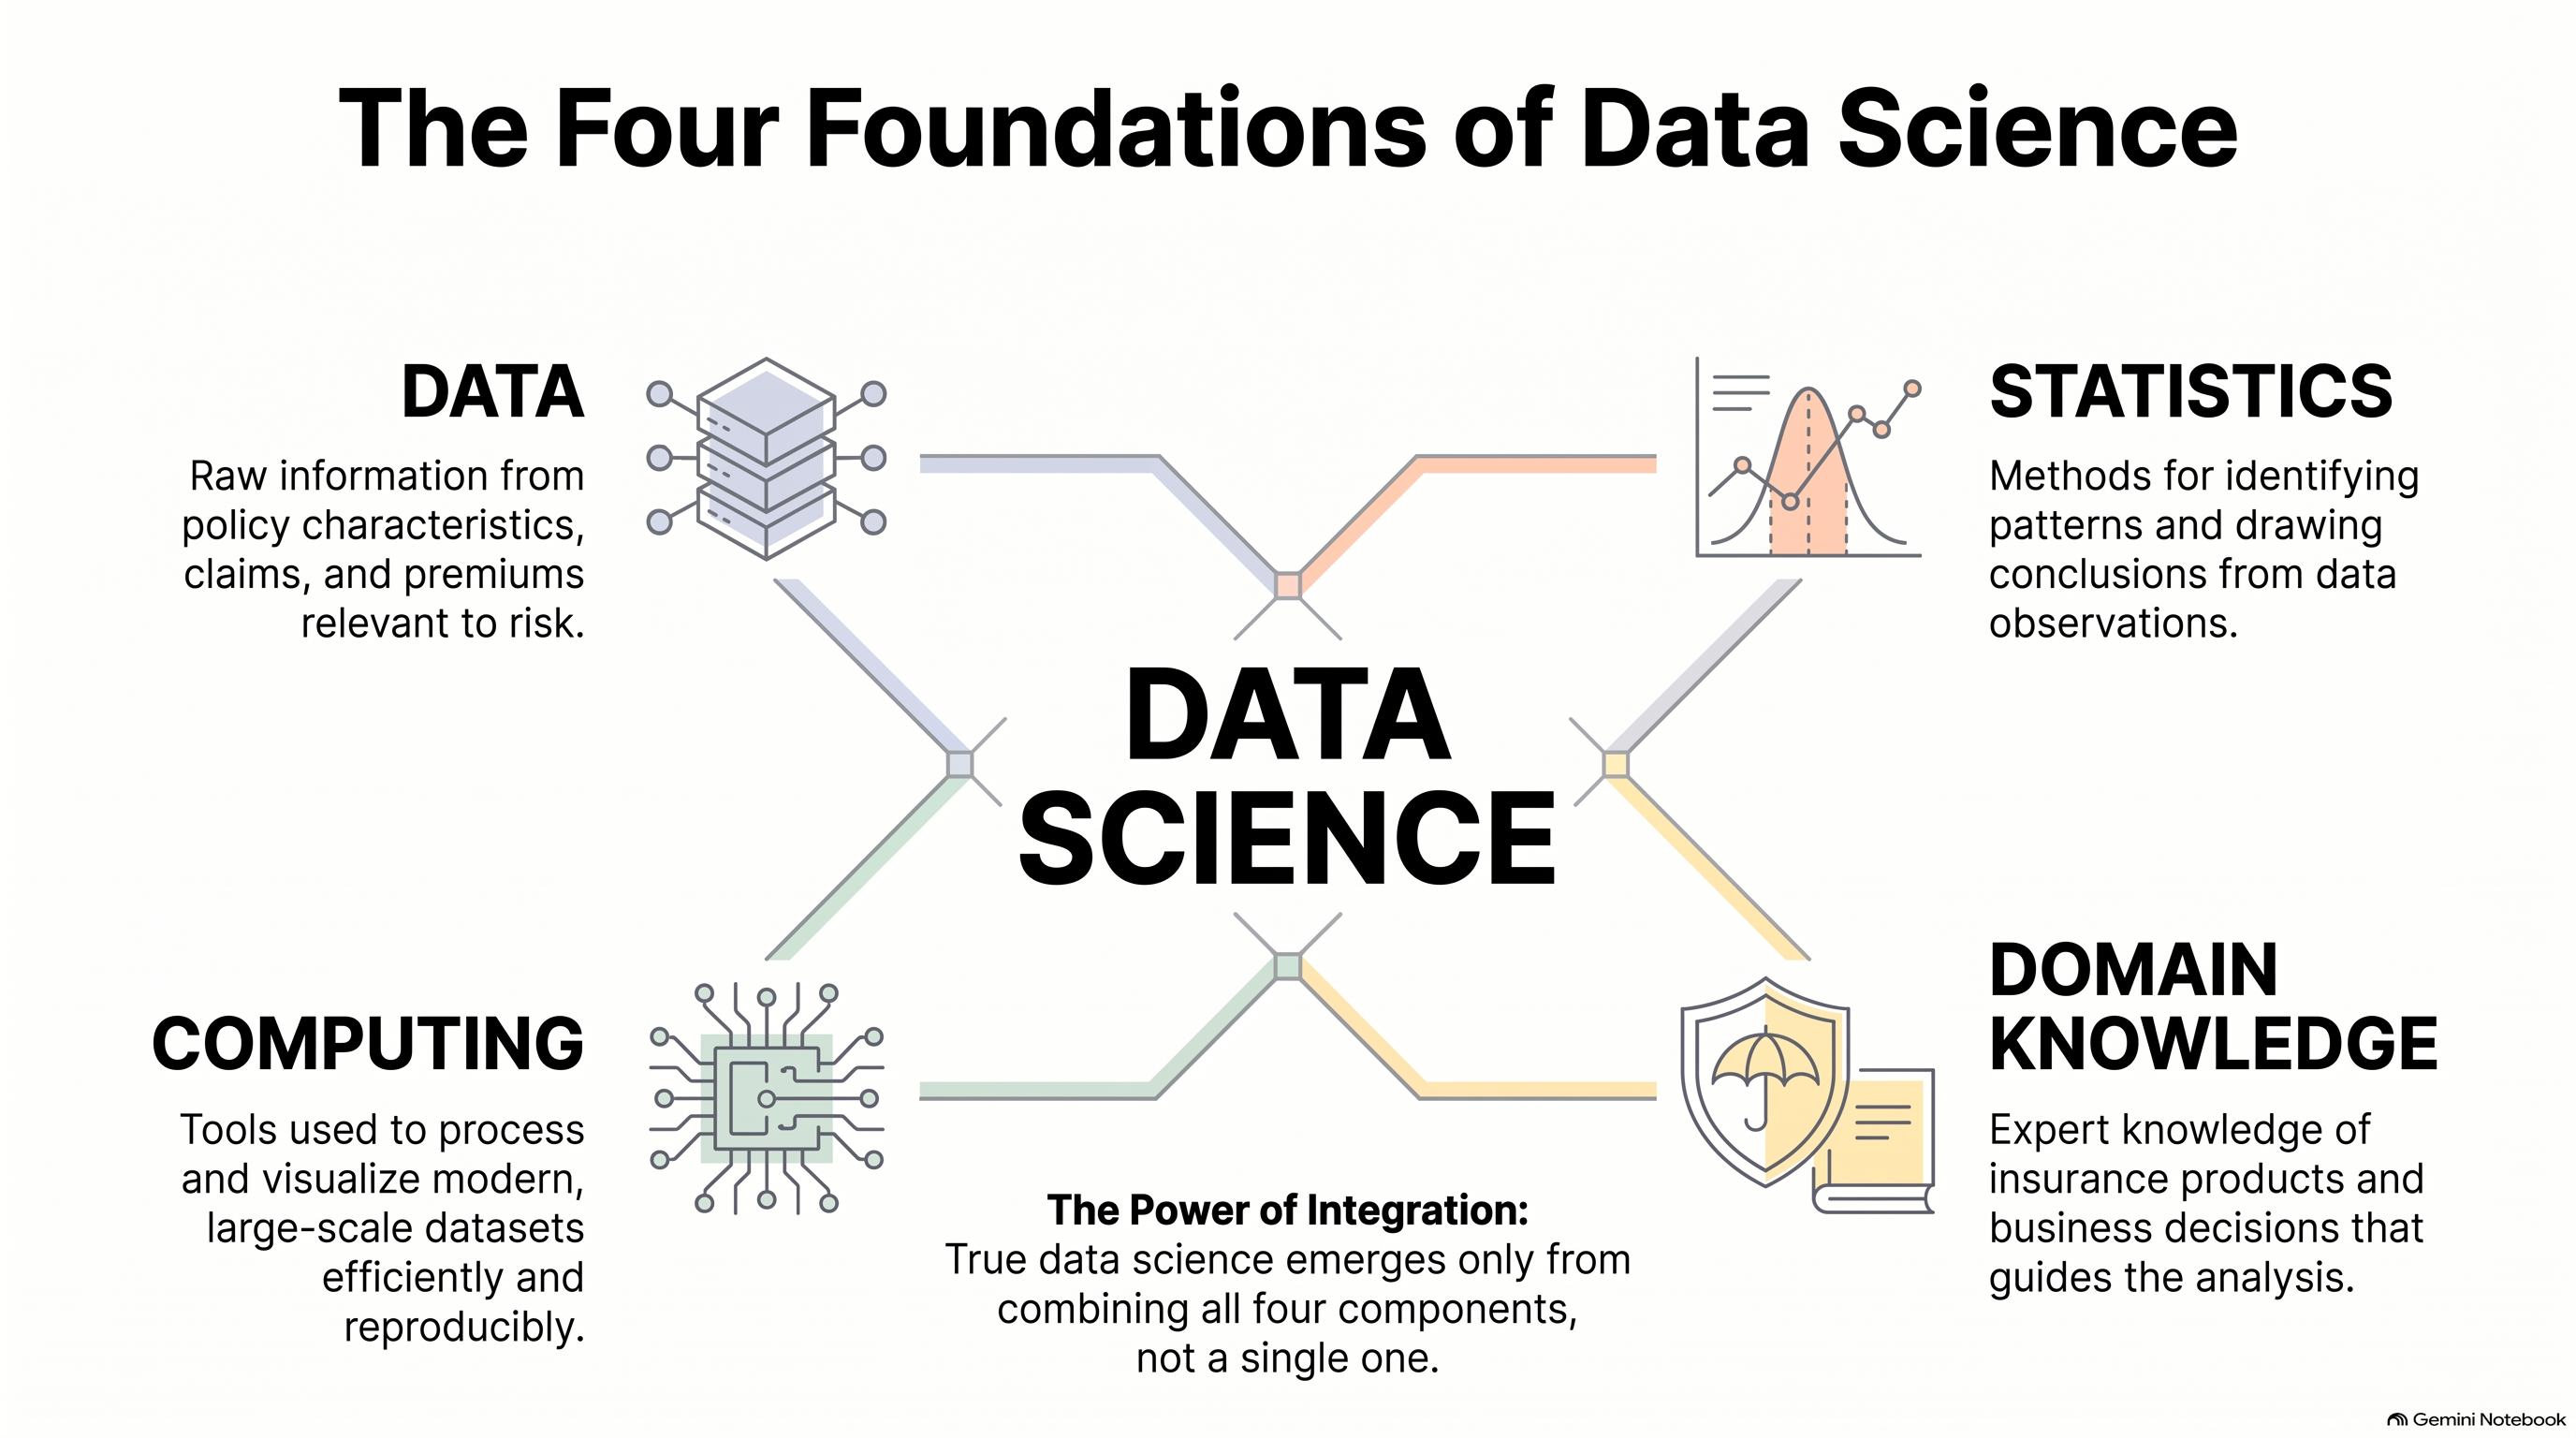
\includegraphics[width=0.85\linewidth,height=\textheight,keepaspectratio]{figures/Four_Foundations_of_Data_Science.png}

}

\caption{\label{fig-foundations-slides}The Four Foundations of Data
Science}

\end{figure}%
\end{frame}

\begin{frame}{Data}
\protect\phantomsection\label{data}
\textbf{Data} provide the observations from which information can be
obtained.

In insurance, data may include:

\begin{itemize}
\tightlist
\item
  policy characteristics;
\item
  exposure;
\item
  claims;
\item
  claim amounts;
\item
  premiums; and
\item
  other information relevant to risk.
\end{itemize}

Without appropriate data, statistical analysis cannot provide useful
evidence about the insurance problem.
\end{frame}

\begin{frame}{Statistics}
\protect\phantomsection\label{statistics}
\textbf{Statistics} provides methods for:

\begin{itemize}
\tightlist
\item
  describing data;
\item
  identifying patterns;
\item
  quantifying uncertainty; and
\item
  drawing conclusions from observations.
\end{itemize}

For example, an insurer may use statistical methods to estimate claim
frequency or compare the experience of different groups.
\end{frame}

\begin{frame}{Computing}
\protect\phantomsection\label{computing}
\textbf{Computing} provides tools for:

\begin{itemize}
\tightlist
\item
  storing data;
\item
  manipulating data;
\item
  analysing data; and
\item
  visualising data.
\end{itemize}

Modern datasets may contain thousands or millions of observations.

Computational tools make it possible to carry out analyses efficiently
and reproducibly.
\end{frame}

\begin{frame}{Domain Knowledge}
\protect\phantomsection\label{domain-knowledge}
\textbf{Domain knowledge} provides an understanding of the context in
which the data arise.

For an actuary, this includes knowledge of:

\begin{itemize}
\tightlist
\item
  insurance products;
\item
  risk;
\item
  exposure;
\item
  claims;
\item
  premiums; and
\item
  the business decisions that the analysis is intended to support.
\end{itemize}
\end{frame}

\begin{frame}{The Four Components Are Complementary}
\protect\phantomsection\label{the-four-components-are-complementary}
The four components work together.

Suppose an insurer observes that one group of policyholders has a higher
claim frequency than another.

\begin{itemize}
\tightlist
\item
  \textbf{Statistics} can quantify the difference.
\item
  \textbf{Computing} can process the underlying data.
\item
  \textbf{Domain knowledge} can determine whether the comparison is
  meaningful.
\item
  \textbf{Data} provide the observations on which the analysis is based.
\end{itemize}

The analysis may also need to account for exposure and other
characteristics that differ between the groups.
\end{frame}

\begin{frame}{Data Science Is More Than Programming}
\protect\phantomsection\label{data-science-is-more-than-programming}
Programming is an important tool in data science.

However, data science is not simply programming with data.

A successful analysis requires:

\begin{itemize}
\tightlist
\item
  an appropriate question;
\item
  reliable data;
\item
  suitable statistical methods; and
\item
  an understanding of the context in which the results will be used.
\end{itemize}

{\def\LTcaptype{none} % do not increment counter
\begin{longtable}[]{@{}
  >{\raggedright\arraybackslash}p{(\linewidth - 4\tabcolsep) * \real{0.3333}}
  >{\raggedright\arraybackslash}p{(\linewidth - 4\tabcolsep) * \real{0.3333}}
  >{\raggedright\arraybackslash}p{(\linewidth - 4\tabcolsep) * \real{0.3333}}@{}}
\toprule\noalign{}
\begin{minipage}[b]{\linewidth}\raggedright
Component
\end{minipage} & \begin{minipage}[b]{\linewidth}\raggedright
Main purpose
\end{minipage} & \begin{minipage}[b]{\linewidth}\raggedright
Example in insurance
\end{minipage} \\
\midrule\noalign{}
\endhead
Data & Provide observations & Policy and claims records \\
Statistics & Quantify and analyse patterns & Estimate claim frequency \\
Computing & Process and analyse data efficiently & Use R to manipulate
and model data \\
Domain knowledge & Interpret results in context & Understand exposure
and insurance risk \\
\bottomrule\noalign{}
\end{longtable}
}
\end{frame}

\begin{frame}{Data Science and Decision-Making}
\protect\phantomsection\label{data-science-and-decision-making}
The ultimate purpose of data science is not to produce tables, graphs,
or models for their own sake.

Its purpose is to provide evidence that can improve decisions.

A useful framework is

\[
\text{Question}
\rightarrow
\text{Data}
\rightarrow
\text{Analysis}
\rightarrow
\text{Evidence}
\rightarrow
\text{Decision}.
\]

For example, an insurer may investigate whether a particular
characteristic should be used in pricing.

The analysis may involve historical policy and claims data, data
preparation, exploration, and statistical modelling.

The resulting evidence can then be considered as part of the pricing
decision.
\end{frame}

\begin{frame}{From Analysis to Action}
\protect\phantomsection\label{from-analysis-to-action}
A useful data-science result should answer three questions:

\begin{enumerate}
\tightlist
\item
  \textbf{What did the data show?}
\item
  \textbf{How reliable is the evidence?}
\item
  \textbf{What decision, if any, should follow from it?}
\end{enumerate}

The quality of a decision depends on more than the predictive
performance of a model.

We must also consider:

\begin{itemize}
\tightlist
\item
  the quality and relevance of the data; assumptions underlying the
  analysis;
\item
  uncertainty in the results; and the consequences of using the results.
\end{itemize}

\begin{tcolorbox}[enhanced jigsaw, arc=.35mm, bottomrule=.15mm, bottomtitle=1mm, breakable, colback=white, colbacktitle=quarto-callout-note-color!10!white, colframe=quarto-callout-note-color-frame, coltitle=black, left=2mm, leftrule=.75mm, opacityback=0, opacitybacktitle=0.6, rightrule=.15mm, title=\textcolor{quarto-callout-note-color}{\faInfo}\hspace{0.5em}{Key idea}, titlerule=0mm, toprule=.15mm, toptitle=1mm]

\textbf{Data science provides analytical evidence; actuarial judgement
provides the insurance context needed to interpret and use that
evidence.}

\end{tcolorbox}
\end{frame}

\subsection{Part III --- The Role of Data in
Insurance}\label{part-iii-the-role-of-data-in-insurance}

\begin{frame}{The Role of Data in Insurance}
\protect\phantomsection\label{the-role-of-data-in-insurance}
Data provide the empirical foundation for many insurance activities.

Insurers collect and maintain information about:

\begin{itemize}
\tightlist
\item
  policies and policyholders;
\item
  exposure;
\item
  premiums;
\item
  claims; and
\item
  payments.
\end{itemize}

These data support decisions about:

\begin{itemize}
\tightlist
\item
  underwriting;
\item
  pricing;
\item
  claims management; and
\item
  risk management.
\end{itemize}
\end{frame}

\begin{frame}{What Makes Insurance Data Useful?}
\protect\phantomsection\label{what-makes-insurance-data-useful}
The usefulness of insurance data depends on more than the amount of
information available.

Data should be:

\begin{itemize}
\tightlist
\item
  relevant to the problem;
\item
  recorded consistently;
\item
  sufficiently complete; and
\item
  sufficiently accurate for the intended analysis.
\end{itemize}

Insurance data must also be interpreted in relation to \textbf{exposure}
and the characteristics of the insurance portfolio.
\end{frame}

\begin{frame}{Why Claim Counts Are Not Enough}
\protect\phantomsection\label{why-claim-counts-are-not-enough}
Suppose two portfolios have:

\begin{itemize}
\tightlist
\item
  Portfolio A: 1,000 claims;
\item
  Portfolio B: 500 claims.
\end{itemize}

We cannot conclude that Portfolio A has twice the claim risk.

Portfolio A may simply have substantially more exposure.

A more meaningful comparison is often based on \textbf{claim frequency}:

\[
\text{Claim frequency}
=
\frac{\text{Number of claims}}
{\text{Exposure}}.
\]

\begin{tcolorbox}[enhanced jigsaw, arc=.35mm, bottomrule=.15mm, bottomtitle=1mm, breakable, colback=white, colbacktitle=quarto-callout-important-color!10!white, colframe=quarto-callout-important-color-frame, coltitle=black, left=2mm, leftrule=.75mm, opacityback=0, opacitybacktitle=0.6, rightrule=.15mm, title=\textcolor{quarto-callout-important-color}{\faExclamation}\hspace{0.5em}{Key idea}, titlerule=0mm, toprule=.15mm, toptitle=1mm]

\textbf{Insurance experience should be interpreted relative to the
amount of exposure.}

Raw counts alone may give a misleading comparison between portfolios.

\end{tcolorbox}
\end{frame}

\begin{frame}{Insurance Data Sources}
\protect\phantomsection\label{insurance-data-sources}
Insurance data come from both \textbf{internal} and \textbf{external}
sources.

Common internal sources include:

\begin{itemize}
\tightlist
\item
  \textbf{Policy data} --- policy type, coverage, dates, insured
  characteristics, and premium.
\item
  \textbf{Exposure data} --- the amount of time or risk exposure
  associated with a policy.
\item
  \textbf{Claims data} --- claim dates, types, status, and amounts.
\item
  \textbf{Payment data} --- premiums, claim payments, expenses, and
  other transactions.
\item
  \textbf{Customer data} --- policyholder characteristics and
  interactions with the insurer.
\end{itemize}
\end{frame}

\begin{frame}{External Data}
\protect\phantomsection\label{external-data}
External sources may provide information relevant to risk assessment.

Examples include:

\begin{itemize}
\tightlist
\item
  geographical information;
\item
  demographic information;
\item
  weather data;
\item
  economic indicators; and
\item
  other publicly or commercially available data.
\end{itemize}

These data may provide information that is not available from the
insurer's own records.
\end{frame}

\begin{frame}{Combining Data Sources}
\protect\phantomsection\label{combining-data-sources}
Insurance information is often stored in different systems.

For example:

\[
\text{Policy system}
\qquad
\text{Claims system}
\qquad
\text{Payment system}
\]

may contain different parts of the information required for an analysis.

These sources may need to be linked using a common identifier, such as a
policy number or claim number.

\[
\text{Policy data}
+
\text{Exposure data}
+
\text{Claims data}
\longrightarrow
\text{Insurance analysis}.
\]
\end{frame}

\begin{frame}{Start with the Question}
\protect\phantomsection\label{start-with-the-question}
The objective of data collection is \textbf{not} to collect as much data
as possible.

The data should be:

\begin{itemize}
\tightlist
\item
  relevant to the question;
\item
  measured appropriately; and
\item
  suitable for the intended analysis.
\end{itemize}

The question should determine which data are required.

\begin{tcolorbox}[enhanced jigsaw, arc=.35mm, bottomrule=.15mm, bottomtitle=1mm, breakable, colback=white, colbacktitle=quarto-callout-note-color!10!white, colframe=quarto-callout-note-color-frame, coltitle=black, left=2mm, leftrule=.75mm, opacityback=0, opacitybacktitle=0.6, rightrule=.15mm, title=\textcolor{quarto-callout-note-color}{\faInfo}\hspace{0.5em}{Start with the question}, titlerule=0mm, toprule=.15mm, toptitle=1mm]

\textbf{Do not begin with ``What data do we have?''}

Begin with:

\begin{quote}
\textbf{What question are we trying to answer?}
\end{quote}

Then determine what data are needed to answer it.

\end{tcolorbox}
\end{frame}

\begin{frame}{Types of Data}
\protect\phantomsection\label{types-of-data}
Insurance datasets contain variables with different characteristics.

Recognising the type of each variable is important because it affects
how the variable can be:

\begin{itemize}
\tightlist
\item
  summarised;
\item
  visualised; and
\item
  analysed.
\end{itemize}

A useful first distinction is between:

\[
\boxed{\text{Categorical data}}
\qquad\text{and}\qquad
\boxed{\text{Numerical data}}.
\]
\end{frame}

\begin{frame}[fragile]{Categorical Data}
\protect\phantomsection\label{categorical-data}
\textbf{Categorical data} describe membership in a group or category.

Examples in insurance include:

\begin{itemize}
\tightlist
\item
  type of insurance;
\item
  geographical area;
\item
  vehicle type;
\item
  policy status; and
\item
  claim type.
\end{itemize}

For example:

\begin{Shaded}
\begin{Highlighting}[]
\NormalTok{Area = Urban}
\NormalTok{Area = Rural}
\end{Highlighting}
\end{Shaded}

The values identify categories rather than numerical quantities.
\end{frame}

\begin{frame}{Numerical Data}
\protect\phantomsection\label{numerical-data}
\textbf{Numerical data} represent quantities for which arithmetic
operations are meaningful.

Examples include:

\begin{itemize}
\tightlist
\item
  age;
\item
  exposure;
\item
  premium;
\item
  number of claims; and
\item
  claim amount.
\end{itemize}

Numerical variables can be further classified as \textbf{discrete} or
\textbf{continuous}.
\end{frame}

\begin{frame}{Discrete and Continuous Data}
\protect\phantomsection\label{discrete-and-continuous-data}
A \textbf{discrete variable} takes values that can be counted.

For example, the number of claims satisfies

\[
N \in {0,1,2,\ldots}.
\]

A \textbf{continuous variable} can take values within an interval.

Examples include:

\begin{itemize}
\tightlist
\item
  claim amount; and
\item
  exposure,
\end{itemize}

depending on how the quantities are measured and recorded.
\end{frame}

\begin{frame}{Structured and Unstructured Data}
\protect\phantomsection\label{structured-and-unstructured-data}
Another useful distinction is between \textbf{structured} and
\textbf{unstructured} data.

\textbf{Structured data} are organised in a predefined format, such as
rows and columns in a database.

Examples:

\begin{itemize}
\tightlist
\item
  policy records;
\item
  claims records; and
\item
  customer databases.
\end{itemize}

\textbf{Unstructured data} do not follow a predefined tabular structure.

Examples include:

\begin{itemize}
\tightlist
\item
  documents;
\item
  images;
\item
  audio; and
\item
  text.
\end{itemize}

For introductory actuarial analysis, structured data are particularly
important.
\end{frame}

\begin{frame}{Types of Insurance Variables}
\protect\phantomsection\label{types-of-insurance-variables}
{\def\LTcaptype{none} % do not increment counter
\begin{longtable}[]{@{}lrl@{}}
\toprule\noalign{}
Variable & Example & Type \\
\midrule\noalign{}
\endhead
Age & 35 & Numerical \\
Area & Urban & Categorical \\
Exposure & 0.75 & Numerical, continuous \\
Number of claims & 2 & Numerical, discrete \\
Claim amount & 18,500 & Numerical \\
Policy status & Active & Categorical \\
\bottomrule\noalign{}
\end{longtable}
}

The classification affects the methods that can be used.

For example:

\begin{itemize}
\tightlist
\item
  numerical distributions can be examined using histograms;
\item
  categorical frequencies can be displayed using bar charts.
\end{itemize}
\end{frame}

\begin{frame}[fragile]{Variable Type and Variable Role}
\protect\phantomsection\label{variable-type-and-variable-role}
The \textbf{type} of a variable and its \textbf{role} in an analysis are
different concepts.

For example, \texttt{Claim\ Amount} may be:

\begin{itemize}
\tightlist
\item
  an outcome variable when modelling claim severity; or
\item
  a variable being summarised during exploratory analysis.
\end{itemize}

Therefore:

\[
\boxed{
\text{Variable type}
\neq
\text{Variable role}
}
\]

The role of a variable depends on the question being investigated.
\end{frame}

\begin{frame}{An Insurance Dataset}
\protect\phantomsection\label{an-insurance-dataset}
Consider the following simplified motor insurance dataset.

Each row represents an insurance policy.

{\def\LTcaptype{none} % do not increment counter
\begin{longtable}[]{@{}rrlrrr@{}}
\toprule\noalign{}
Policy & Age & Area & Exposure & Claims & Claim Amount \\
\midrule\noalign{}
\endhead
1 & 24 & Urban & 1.00 & 1 & 12,500 \\
2 & 42 & Rural & 1.00 & 0 & 0 \\
3 & 31 & Urban & 0.50 & 2 & 8,400 \\
4 & 56 & Rural & 1.00 & 0 & 0 \\
5 & 27 & Urban & 0.75 & 1 & 21,300 \\
6 & 45 & Urban & 1.00 & 0 & 0 \\
\bottomrule\noalign{}
\end{longtable}
}
\end{frame}

\begin{frame}[fragile]{Reading the Dataset}
\protect\phantomsection\label{reading-the-dataset}
Different variables describe different aspects of the insurance risk.

\begin{itemize}
\tightlist
\item
  \texttt{Age} describes a characteristic of the policyholder.
\item
  \texttt{Area} describes the geographical category.
\item
  \texttt{Exposure} describes the amount of risk observed.
\item
  \texttt{Claims} records the number of observed claims.
\item
  \texttt{Claim\ Amount} records the aggregate claim amount.
\end{itemize}

The same dataset can therefore be used to investigate several different
questions.
\end{frame}

\begin{frame}{Questions from the Dataset}
\protect\phantomsection\label{questions-from-the-dataset}
\textbf{Descriptive question}

\begin{quote}
How does claim experience vary across different areas?
\end{quote}

\textbf{Frequency question}

\begin{quote}
What is the observed claim frequency?
\end{quote}

\textbf{Severity question}

\begin{quote}
What is the average claim amount among policies with claims?
\end{quote}

\textbf{Comparative question}

\begin{quote}
Does claim experience appear to differ between younger and older
policyholders?
\end{quote}

Different questions may require different summaries and analytical
methods.
\end{frame}

\begin{frame}{Frequency and Severity}
\protect\phantomsection\label{frequency-and-severity}
Two fundamental quantities in insurance analysis are \textbf{claim
frequency} and \textbf{claim severity}.

Claim frequency measures the number of claims relative to exposure:

\[
\text{Claim frequency}
=\frac{\text{Number of claims}}
{\text{Exposure}}.
\]

Average claim severity measures the average claim amount among claims:

\[
\text{Average severity}
=\frac{\text{Total claim amount}}
{\text{Number of claims}},
\]

provided that the denominator is positive.
\end{frame}

\begin{frame}{Frequency x Severity}
\protect\phantomsection\label{frequency-x-severity}
The two quantities can be combined to obtain a simple measure of
expected loss per unit exposure:

\[
\text{Expected loss per unit exposure}
\approx
\text{Claim frequency}
\times
\text{Average severity}.
\]

This provides a simple bridge between insurance concepts and data
science.

The quantities are estimated from observed data.

More advanced methods can then investigate how frequency and severity
vary with risk characteristics.

\begin{tcolorbox}[enhanced jigsaw, arc=.35mm, bottomrule=.15mm, bottomtitle=1mm, breakable, colback=white, colbacktitle=quarto-callout-note-color!10!white, colframe=quarto-callout-note-color-frame, coltitle=black, left=2mm, leftrule=.75mm, opacityback=0, opacitybacktitle=0.6, rightrule=.15mm, title=\textcolor{quarto-callout-note-color}{\faInfo}\hspace{0.5em}{Key idea}, titlerule=0mm, toprule=.15mm, toptitle=1mm]

Insurance data contain different types of information about a risk.

\textbf{Frequency} describes how often claims occur, while
\textbf{severity} describes the size of claims.

Both are needed to understand insurance losses.

\end{tcolorbox}
\end{frame}

\subsection{Part IV --- The Data Science Life
Cycle}\label{part-iv-the-data-science-life-cycle}

\begin{frame}{The Data Science Life Cycle}
\protect\phantomsection\label{the-data-science-life-cycle}
A data science project transforms a practical problem into an
evidence-based decision.

Although individual projects differ, most involve several common stages:

\begin{figure}

\centering{

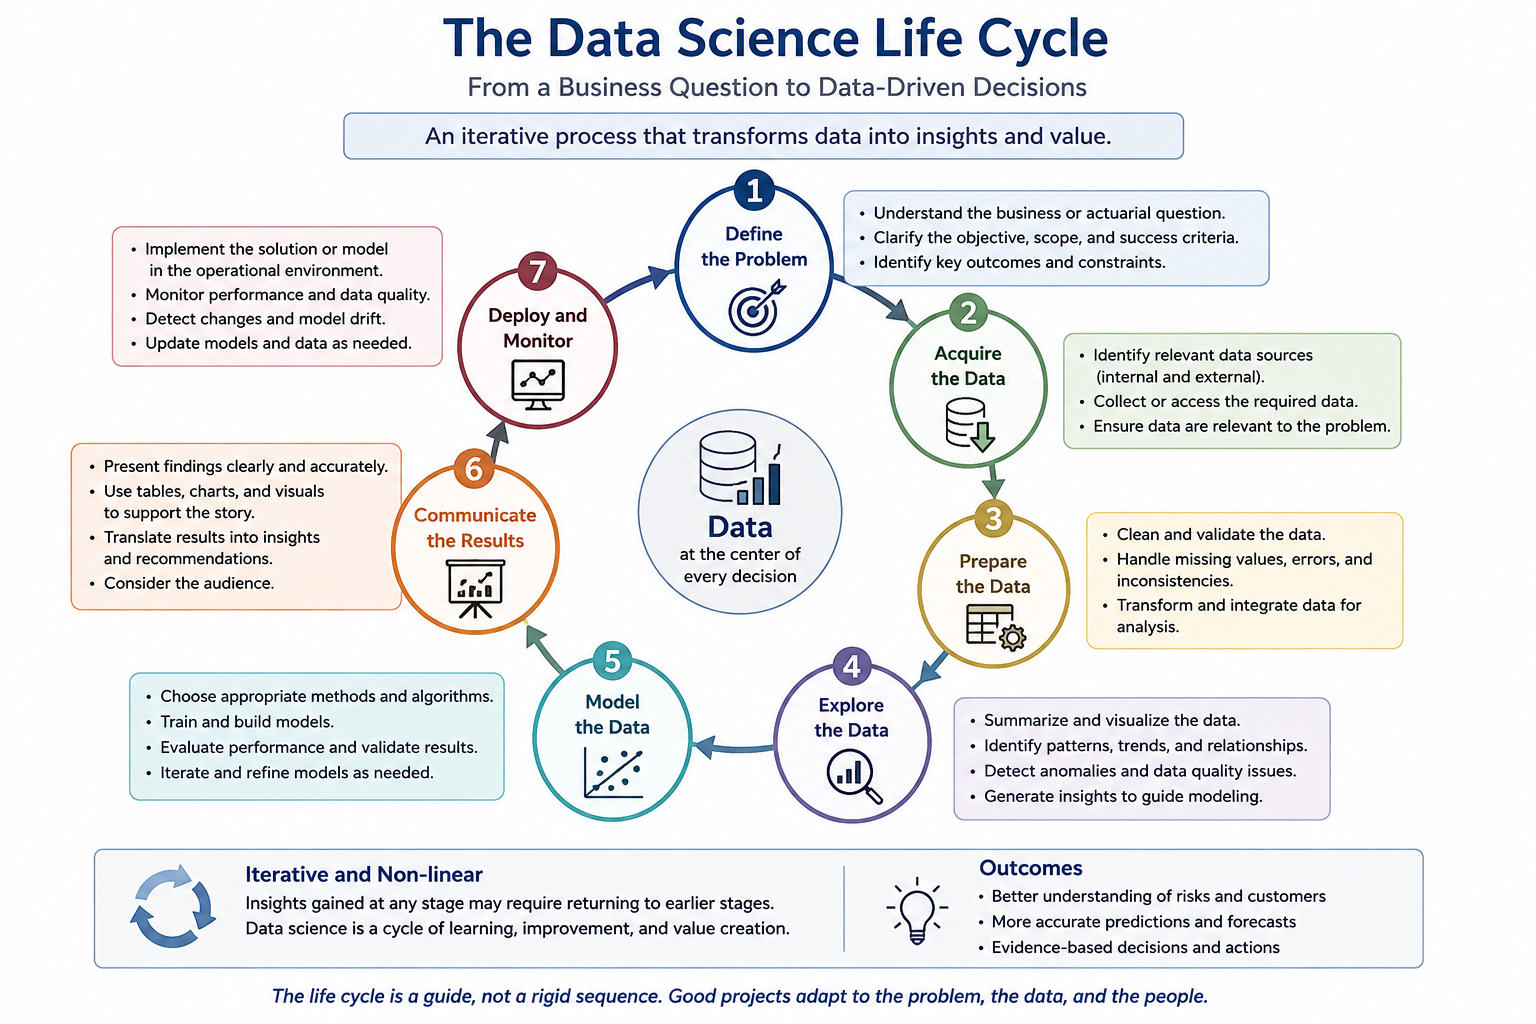
\includegraphics[width=0.6\linewidth,height=\textheight,keepaspectratio]{figures/Data_Science_Life_Cycle.png}

}

\caption{\label{fig-lifecycle-slides}Data Science Life Cycle}

\end{figure}%
\end{frame}

\begin{frame}{The Life Cycle Is Not Strictly Linear}
\protect\phantomsection\label{the-life-cycle-is-not-strictly-linear}
The stages provide a framework for organising a data science project.

They should not be viewed as a strictly linear sequence.

For example:

\begin{itemize}
\tightlist
\item
  exploration may reveal data-quality problems;
\item
  data preparation may require returning to the data source;
\item
  modelling may reveal that the original question needs reconsideration;
  and
\item
  monitoring may show that a deployed model needs to be updated.
\end{itemize}

\[
\boxed{\text{Data science is a cycle, not a one-time process.}}
\]
\end{frame}

\begin{frame}{1. Define the Problem}
\protect\phantomsection\label{define-the-problem}
A data science project should begin with a \textbf{question or
decision}.

It should not begin simply because a dataset or a modelling technique is
available.

For an insurance problem, we should establish:

\begin{itemize}
\tightlist
\item
  what decision needs to be supported;
\item
  what outcome is of interest;
\item
  which population or portfolio is being studied;
\item
  what information may be relevant; and
\item
  how the results will be used.
\end{itemize}
\end{frame}

\begin{frame}{Example: Defining an Insurance Problem}
\protect\phantomsection\label{example-defining-an-insurance-problem}
Suppose an insurer observes differences in motor insurance claim
experience.

A useful question is:

\begin{quote}
\textbf{Which characteristics are associated with differences in claim
frequency?}
\end{quote}

This is more informative than:

\begin{quote}
``We want to analyse the claims data.''
\end{quote}

The first question identifies the outcome of interest and gives
direction to the analysis.
\end{frame}

\begin{frame}{From Question to Measurable Quantities}
\protect\phantomsection\label{from-question-to-measurable-quantities}
A practical question must be translated into quantities that can be
measured using data.

For claim frequency, we need information about:

\begin{itemize}
\tightlist
\item
  the number of claims; and
\item
  the corresponding exposure.
\end{itemize}

Thus,

\[
\text{Question}
\rightarrow
\text{Measurable outcome}
\rightarrow
\text{Required data}.
\]

\begin{tcolorbox}[enhanced jigsaw, arc=.35mm, bottomrule=.15mm, bottomtitle=1mm, breakable, colback=white, colbacktitle=quarto-callout-important-color!10!white, colframe=quarto-callout-important-color-frame, coltitle=black, left=2mm, leftrule=.75mm, opacityback=0, opacitybacktitle=0.6, rightrule=.15mm, title=\textcolor{quarto-callout-important-color}{\faExclamation}\hspace{0.5em}{Start with the decision, not the model}, titlerule=0mm, toprule=.15mm, toptitle=1mm]

The choice of statistical or machine-learning method should follow from
the problem.

A sophisticated model is not useful if it does not answer a relevant
question or support a meaningful decision.

\end{tcolorbox}
\end{frame}

\begin{frame}{2. Acquire the Data}
\protect\phantomsection\label{acquire-the-data}
Once the problem has been defined, the next stage is to obtain the
required data.

Insurance data may come from:

\begin{itemize}
\tightlist
\item
  policy administration systems;
\item
  claims systems;
\item
  financial records;
\item
  customer databases; and
\item
  external sources.
\end{itemize}

Data from different systems may need to be combined using a common
identifier.
\end{frame}

\begin{frame}{What Data Are Required?}
\protect\phantomsection\label{what-data-are-required}
The required data depend on the question.

For example, analysing claim frequency may require:

\begin{itemize}
\tightlist
\item
  number of claims;
\item
  exposure;
\item
  policy characteristics; and
\item
  relevant risk characteristics.
\end{itemize}

Data acquisition may involve:

\begin{itemize}
\tightlist
\item
  importing files;
\item
  querying databases;
\item
  accessing APIs; or
\item
  obtaining data from external sources.
\end{itemize}
\end{frame}

\begin{frame}{Available Data vs Appropriate Data}
\protect\phantomsection\label{available-data-vs-appropriate-data}
Having a large dataset does not guarantee a useful analysis.

We must distinguish between:

\[
\boxed{\text{Available data}}
\qquad\text{and}\qquad
\boxed{\text{Appropriate data}}.
\]

Data are appropriate when they measure quantities relevant to the
problem and are suitable for the intended analysis.
\end{frame}

\begin{frame}{3. Prepare the Data}
\protect\phantomsection\label{prepare-the-data}
Raw data are rarely ready for analysis.

\textbf{Data preparation} involves:

\begin{itemize}
\tightlist
\item
  checking;
\item
  cleaning;
\item
  transforming; and
\item
  organising the data.
\end{itemize}

Common problems include:

\begin{itemize}
\tightlist
\item
  missing values;
\item
  invalid or impossible values;
\item
  inconsistent data types;
\item
  duplicated observations;
\item
  inconsistent categories;
\item
  incorrect dates; and
\item
  observations outside the relevant period.
\end{itemize}
\end{frame}

\begin{frame}{Data Preparation in Insurance}
\protect\phantomsection\label{data-preparation-in-insurance}
Insurance data provide many examples.

For example:

\begin{itemize}
\tightlist
\item
  a policy may have a missing inception date;
\item
  an exposure period may be incorrectly recorded;
\item
  a claim may be linked to an inactive policy; or
\item
  the same geographical area may appear under different labels.
\end{itemize}

These problems can affect the results of subsequent analysis.
\end{frame}

\begin{frame}{Data Transformation}
\protect\phantomsection\label{data-transformation}
Data preparation may also require transformations.

For example:

\begin{itemize}
\tightlist
\item
  converting dates into a standard format; standardising category
  labels; or
\item
  aggregating several claim records to obtain total claim amount by
  policy.
\end{itemize}

The objective is not simply to make the dataset look tidy.

Each transformation should have a clear reason based on:

\begin{itemize}
\tightlist
\item
  the meaning of the data; and the requirements of the analysis.
\end{itemize}

\begin{tcolorbox}[enhanced jigsaw, arc=.35mm, bottomrule=.15mm, bottomtitle=1mm, breakable, colback=white, colbacktitle=quarto-callout-note-color!10!white, colframe=quarto-callout-note-color-frame, coltitle=black, left=2mm, leftrule=.75mm, opacityback=0, opacitybacktitle=0.6, rightrule=.15mm, title=\textcolor{quarto-callout-note-color}{\faInfo}\hspace{0.5em}{Data cleaning is part of the analysis}, titlerule=0mm, toprule=.15mm, toptitle=1mm]

Decisions about missing, invalid, or unusual observations can affect the
results.

Data preparation should therefore be documented and carried out with an
understanding of the underlying insurance process.

\end{tcolorbox}
\end{frame}

\begin{frame}{4. Explore the Data}
\protect\phantomsection\label{explore-the-data}
After the data have been prepared, the next stage is \textbf{exploratory
data analysis (EDA)}.

The purpose of EDA is to understand the main characteristics of the data
before formal modelling.

EDA can examine:

\begin{itemize}
\tightlist
\item
  distributions of variables;
\item
  differences between groups;
\item
  relationships between variables;
\item
  unusual or extreme observations;
\item
  missing values; and
\item
  possible data-quality problems.
\end{itemize}
\end{frame}

\begin{frame}{Numerical and Graphical Exploration}
\protect\phantomsection\label{numerical-and-graphical-exploration}
EDA uses both numerical summaries and graphical methods.

\textbf{Numerical summaries} include:

\begin{itemize}
\tightlist
\item
  mean;
\item
  median;
\item
  standard deviation; and
\item
  other descriptive statistics.
\end{itemize}

\textbf{Graphical methods} include:

\begin{itemize}
\tightlist
\item
  histograms;
\item
  boxplots;
\item
  bar charts; and
\item
  scatterplots.
\end{itemize}

Different methods reveal different features of the data.
\end{frame}

\begin{frame}{EDA in Insurance}
\protect\phantomsection\label{eda-in-insurance}
Suppose an insurer wants to understand differences in claim experience.

EDA might be used to:

\begin{itemize}
\tightlist
\item
  compare claim frequency across geographical areas;
\item
  examine the distribution of claim amounts;
\item
  identify unusually large claims; and
\item
  investigate relationships between age and claim experience.
\end{itemize}

EDA can reveal patterns that require further investigation.
\end{frame}

\begin{frame}{EDA Before Modelling}
\protect\phantomsection\label{eda-before-modelling}
Exploration is more than a preliminary presentation of the data.

It may reveal:

\begin{itemize}
\tightlist
\item
  variables that require transformation;
\item
  groups that should be examined separately;
\item
  unusual observations; or
\item
  relationships that require further investigation.
\end{itemize}

Thus,

\[
\boxed{
\text{Explore}
\rightarrow
\text{Understand}
\rightarrow
\text{Model}
}
\]

The analysis should be guided by what the data can reasonably support.
\end{frame}

\begin{frame}{5. Model the Data}
\protect\phantomsection\label{model-the-data}
When modelling is required, an appropriate statistical or computational
model can be developed.

A model provides a mathematical representation of relationships in the
data.

Depending on the problem, the objective may be to:

\begin{itemize}
\tightlist
\item
  explain observed patterns;
\item
  estimate an unknown quantity; or
\item
  predict future outcomes.
\end{itemize}
\end{frame}

\begin{frame}{Insurance Modelling Examples}
\protect\phantomsection\label{insurance-modelling-examples}
Data science models can be used for:

\begin{itemize}
\tightlist
\item
  claim frequency;
\item
  claim severity;
\item
  probability of a claim;
\item
  future claims; and
\item
  expected losses.
\end{itemize}

The appropriate model depends on:

\begin{itemize}
\tightlist
\item
  the nature of the outcome;
\item
  the available data;
\item
  the purpose of the analysis; and
\item
  the assumptions that can reasonably be made.
\end{itemize}
\end{frame}

\begin{frame}{Different Outcomes Require Different Models}
\protect\phantomsection\label{different-outcomes-require-different-models}
The number of claims is a \textbf{count variable}.

Claim amount is a \textbf{monetary variable}.

These outcomes have different characteristics and may therefore require
different modelling approaches.

The model should follow from the problem and the nature of the data.
\end{frame}

\begin{frame}{Model Evaluation}
\protect\phantomsection\label{model-evaluation}
Model development should include evaluation.

A model that fits historical data well may not necessarily provide
reliable predictions for new observations.

Therefore, we need to assess whether the model is:

\begin{itemize}
\tightlist
\item
  appropriate for the problem;
\item
  consistent with its assumptions; and
\item
  useful for its intended purpose.
\end{itemize}

\begin{tcolorbox}[enhanced jigsaw, arc=.35mm, bottomrule=.15mm, bottomtitle=1mm, breakable, colback=white, colbacktitle=quarto-callout-important-color!10!white, colframe=quarto-callout-important-color-frame, coltitle=black, left=2mm, leftrule=.75mm, opacityback=0, opacitybacktitle=0.6, rightrule=.15mm, title=\textcolor{quarto-callout-important-color}{\faExclamation}\hspace{0.5em}{A model is an approximation}, titlerule=0mm, toprule=.15mm, toptitle=1mm]

A statistical model does not reproduce reality exactly.

It provides a simplified representation of relationships observed in the
data.

Its usefulness depends on whether its assumptions and results are
appropriate for the problem being considered.

\end{tcolorbox}
\end{frame}

\begin{frame}{6. Communicate the Results}
\protect\phantomsection\label{communicate-the-results}
The results of an analysis must be communicated clearly to the people
who will use them.

A technically correct analysis has limited value if its findings cannot
be understood or connected to the original decision.

Communication may involve:

\begin{itemize}
\tightlist
\item
  tables;
\item
  charts and visualisations;
\item
  written reports;
\item
  presentations; or
\item
  interactive dashboards.
\end{itemize}
\end{frame}

\begin{frame}{Communicate for the Audience}
\protect\phantomsection\label{communicate-for-the-audience}
The form of communication should reflect the audience.

For example:

\textbf{Actuarial report}

\begin{itemize}
\tightlist
\item
  assumptions;
\item
  methodology;
\item
  model performance; and
\item
  technical interpretation.
\end{itemize}

\textbf{Senior management}

\begin{itemize}
\tightlist
\item
  main findings;
\item
  important limitations; and
\item
  implications for the decision.
\end{itemize}

The same analysis may therefore require different forms of
communication.
\end{frame}

\begin{frame}{From Results to Decisions}
\protect\phantomsection\label{from-results-to-decisions}
Good communication should connect the results back to the original
question.

For example, instead of simply reporting:

\begin{quote}
Group A has a higher observed claim frequency than Group B.
\end{quote}

the analysis should explain:

\begin{itemize}
\tightlist
\item
  the size of the difference;
\item
  the evidence supporting it;
\item
  relevant limitations; and
\item
  possible implications for the insurance decision.
\end{itemize}

A useful structure is:

\[
\text{Problem}
\rightarrow
\text{Evidence}
\rightarrow
\text{Interpretation}
\rightarrow
\text{Implication}.
\]
\end{frame}

\begin{frame}{7. Deploy and Monitor}
\protect\phantomsection\label{deploy-and-monitor}
When a model is intended for operational use, the final stage is to
\textbf{deploy and monitor} it.

\textbf{Deployment} means making the model available within the process
for which it was developed.

For example, a predictive model might be incorporated into an
underwriting system to estimate risk when a new policy is quoted.
\end{frame}

\begin{frame}{Before Deployment}
\protect\phantomsection\label{before-deployment}
Deployment should normally be preceded by appropriate testing.

The model should be checked in an environment that reflects its intended
use before it is introduced into production.

The objective is to ensure that the model behaves as expected when used
in practice.
\end{frame}

\begin{frame}{Why Monitoring Is Necessary}
\protect\phantomsection\label{why-monitoring-is-necessary}
A deployed model should not simply be left unchanged.

Over time, the following may change:

\begin{itemize}
\tightlist
\item
  insurance portfolios;
\item
  customer behaviour;
\item
  economic conditions;
\item
  claim patterns; and
\item
  data-generation processes.
\end{itemize}

A model that performed well when developed may therefore become less
appropriate later.
\end{frame}

\begin{frame}{What Should Be Monitored?}
\protect\phantomsection\label{what-should-be-monitored}
Monitoring may include:

\begin{itemize}
\tightlist
\item
  predictive performance;
\item
  data quality;
\item
  unusual changes in input variables; and
\item
  differences between predicted and observed outcomes.
\end{itemize}

For example, suppose a claim prediction model consistently
underestimates claim frequency for a particular segment.

The model may need to be:

\begin{itemize}
\tightlist
\item
  investigated;
\item
  recalibrated; or
\item
  redeveloped.
\end{itemize}
\end{frame}

\begin{frame}{The Complete Life Cycle}
\protect\phantomsection\label{the-complete-life-cycle}
The complete process is:

\[
\boxed{
\text{Define}
\rightarrow
\text{Acquire}
\rightarrow
\text{Prepare}
\rightarrow
\text{Explore}
\rightarrow
\text{Model}
\rightarrow
\text{Communicate}
\rightarrow
\text{Deploy and Monitor}
}
\]

However, the process does not end with deployment.

Monitoring can lead back to earlier stages.
\end{frame}

\begin{frame}{The Life Cycle Is Iterative}
\protect\phantomsection\label{the-life-cycle-is-iterative}
For example:

\[
\text{Monitor}
\rightarrow
\text{New problem}
\rightarrow
\text{New data}
\rightarrow
\text{New analysis}.
\]

Similarly:

\[
\text{Explore}
\rightarrow
\text{Data-quality problem}
\rightarrow
\text{Prepare again}.
\]

\[
\text{Model}
\rightarrow
\text{Poor performance}
\rightarrow
\text{Reconsider the model or data}.
\]

\begin{tcolorbox}[enhanced jigsaw, arc=.35mm, bottomrule=.15mm, bottomtitle=1mm, breakable, colback=white, colbacktitle=quarto-callout-note-color!10!white, colframe=quarto-callout-note-color-frame, coltitle=black, left=2mm, leftrule=.75mm, opacityback=0, opacitybacktitle=0.6, rightrule=.15mm, title=\textcolor{quarto-callout-note-color}{\faInfo}\hspace{0.5em}{Key idea}, titlerule=0mm, toprule=.15mm, toptitle=1mm]

\textbf{Data science is a cycle, not a one-time process.}

The objective is to develop solutions that remain useful as the data,
environment, and decision-making requirements change.

\end{tcolorbox}
\end{frame}

\begin{frame}{From an Insurance Question to a Decision}
\protect\phantomsection\label{from-an-insurance-question-to-a-decision}
The life cycle can be viewed as a continuous process:

\[
\boxed{
\text{Insurance Question}
\rightarrow
\text{Data}
\rightarrow
\text{Analysis}
\rightarrow
\text{Evidence}
\rightarrow
\text{Actuarial Judgement}
\rightarrow
\text{Decision}
\circlearrowleft
}
\]

Each stage contributes to turning an insurance problem into an
evidence-based decision.
\end{frame}

\subsection{Part V --- Roles in a Data Science
Team}\label{part-v-roles-in-a-data-science-team}

\begin{frame}{Roles in a Data Science Team}
\protect\phantomsection\label{roles-in-a-data-science-team}
Data science projects often involve people with different areas of
expertise.

The responsibilities may overlap, especially in smaller organisations,
but different roles typically contribute different skills.

Common roles include:

\begin{itemize}
\tightlist
\item
  \textbf{Data analyst} --- understands and communicates information in
  data.
\item
  \textbf{Data scientist} --- develops analytical and predictive models.
\item
  \textbf{Data engineer} --- builds and maintains data infrastructure.
\item
  \textbf{Actuary} --- applies risk and insurance expertise to the
  problem.
\end{itemize}
\end{frame}

\begin{frame}{Data Science Team Roles}
\protect\phantomsection\label{data-science-team-roles}
\begin{figure}

\centering{

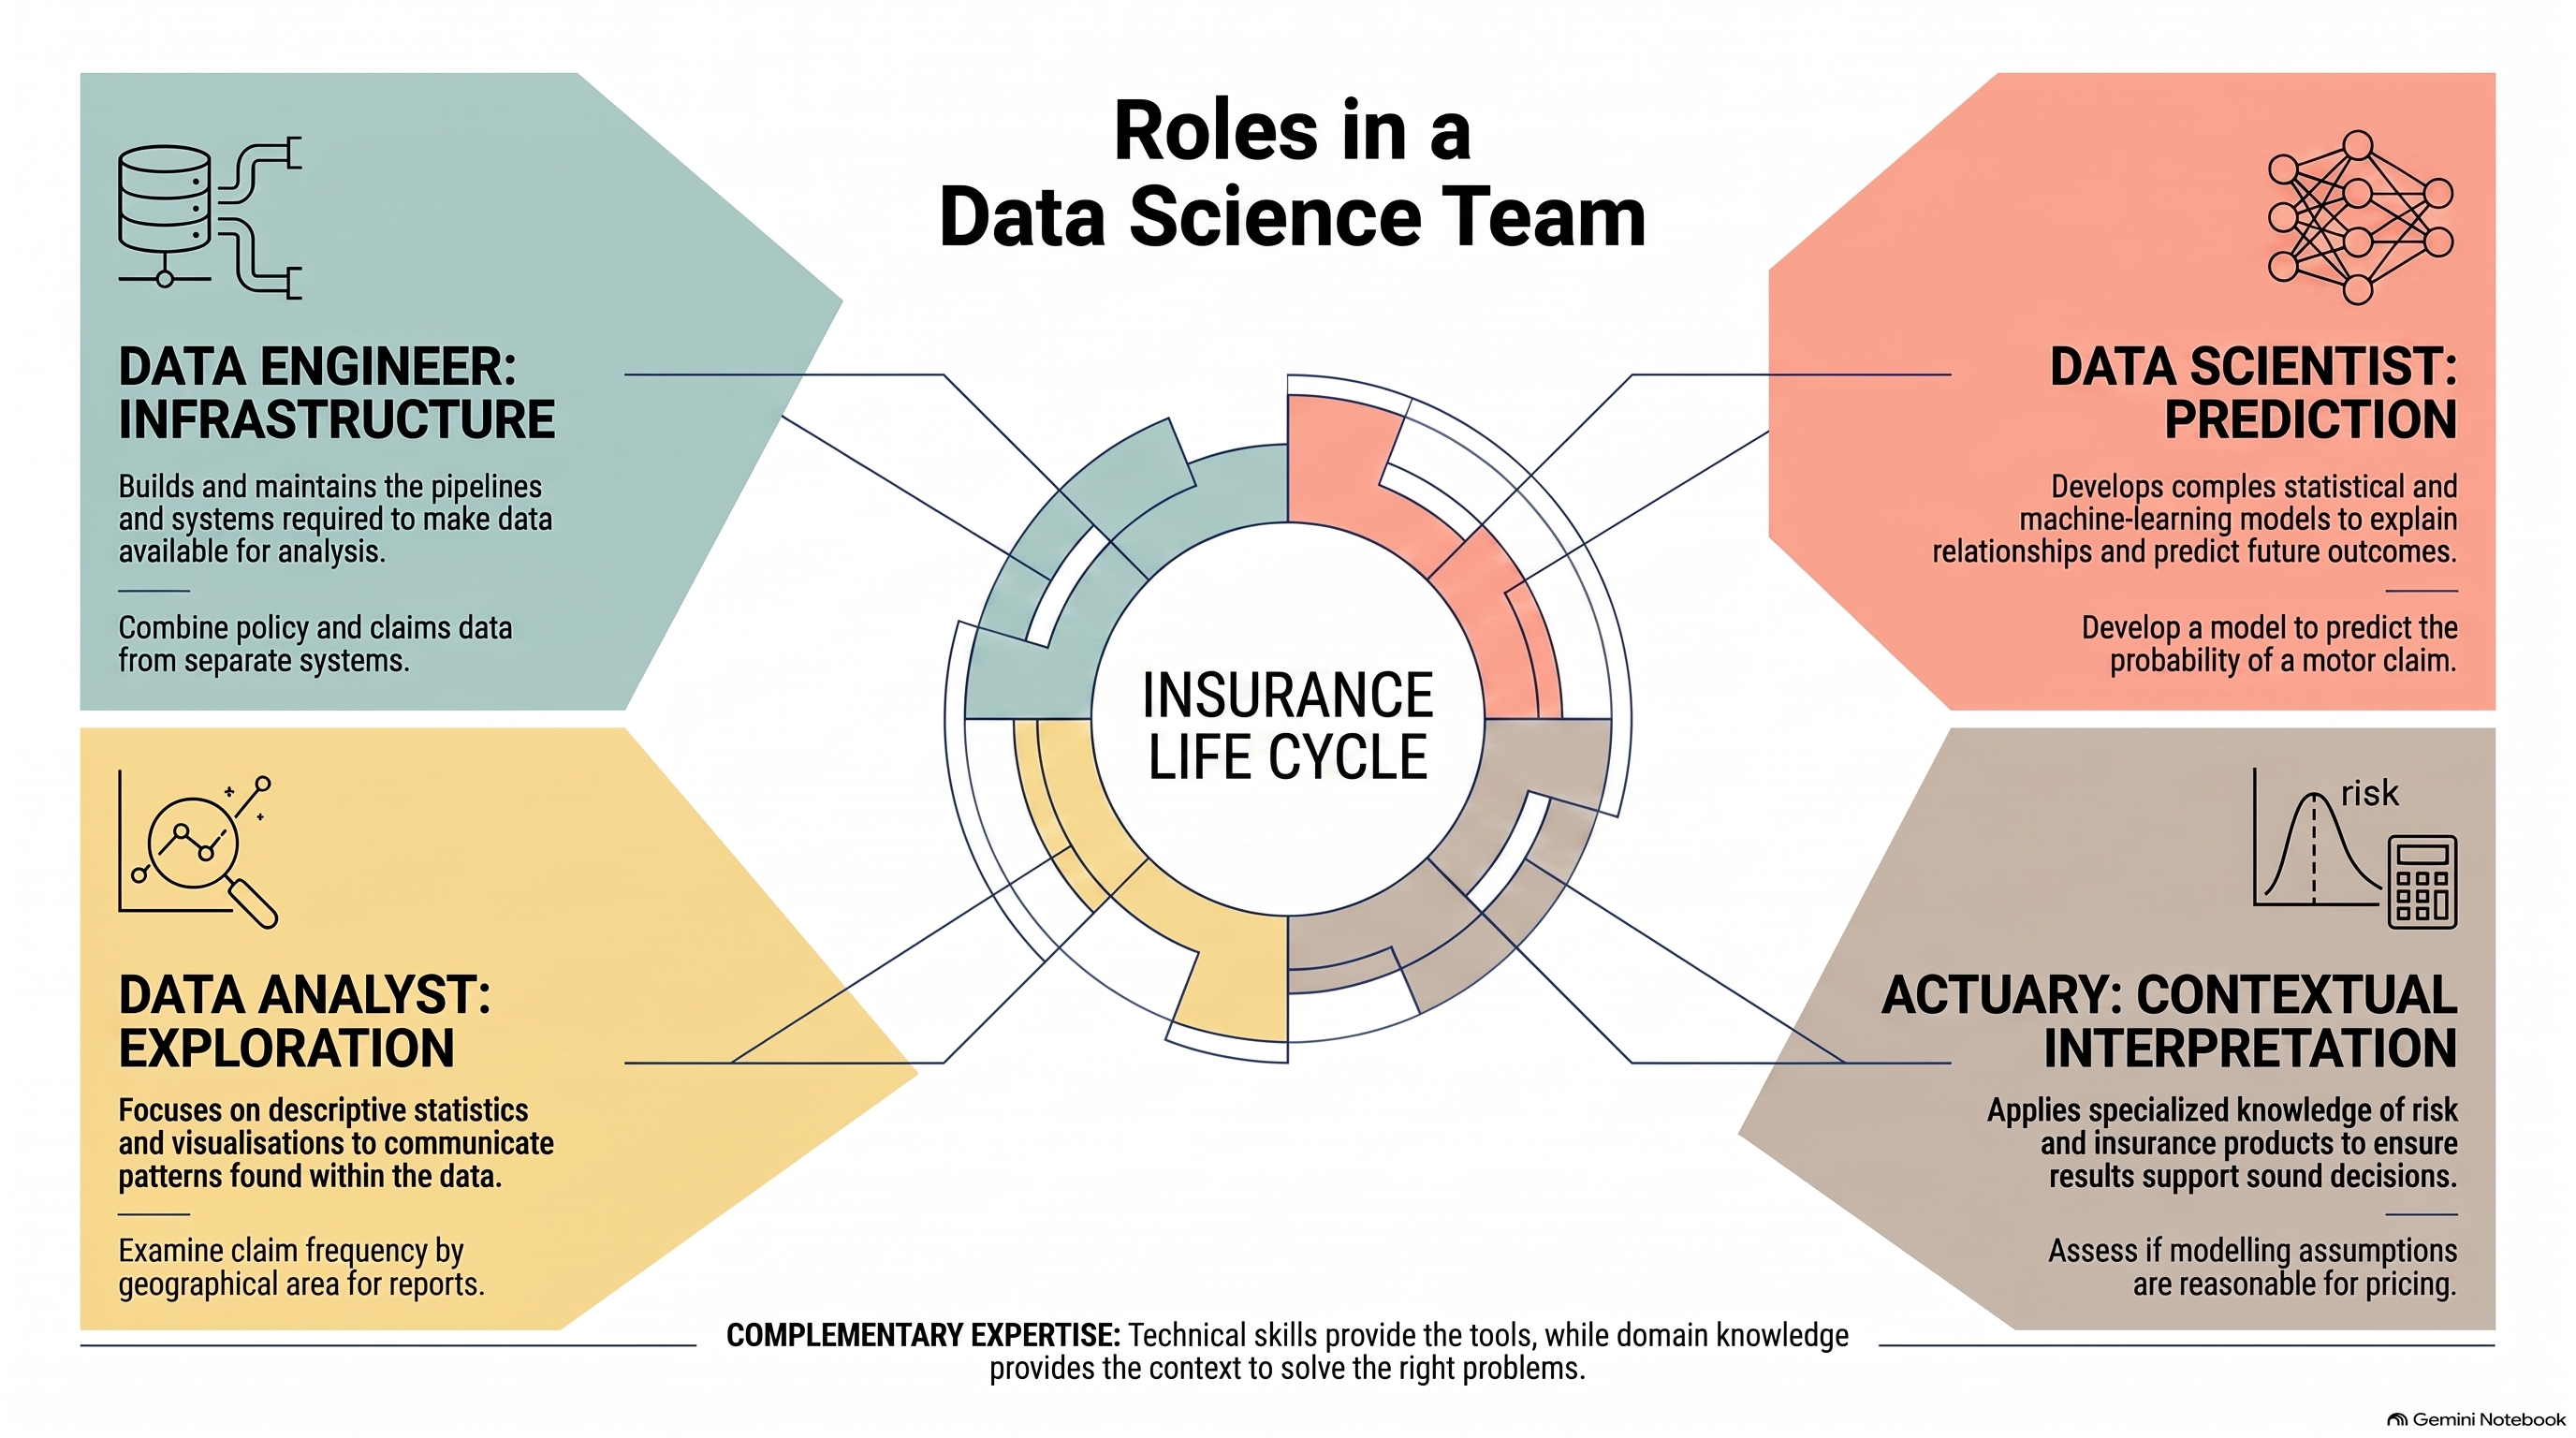
\includegraphics[width=0.85\linewidth,height=\textheight,keepaspectratio]{figures/Data_Science_Team_Roles.png}

}

\caption{\label{fig-team-roles-slides}Core Roles and Responsibilities in
a Data Science Team}

\end{figure}%

The exact responsibilities depend on the organisation.

In a small organisation, one person may perform several roles.

In a larger organisation, responsibilities may be distributed among
specialists.
\end{frame}

\begin{frame}{Data Analyst}
\protect\phantomsection\label{data-analyst}
A \textbf{data analyst} focuses on understanding and communicating
information contained in data.

Typical activities include:

\begin{itemize}
\tightlist
\item
  preparing data for analysis;
\item
  producing descriptive statistics;
\item
  identifying patterns and trends;
\item
  creating tables and visualisations; and
\item
  communicating findings to stakeholders.
\end{itemize}

For example, an insurance data analyst might examine claim frequency by
geographical area and report differences in observed experience.

The role is closely associated with the \textbf{exploration and
communication} stages of the data science life cycle.
\end{frame}

\begin{frame}{Data Scientist}
\protect\phantomsection\label{data-scientist}
A \textbf{data scientist} typically works on more complex analytical and
predictive problems.

The role may involve:

\begin{itemize}
\tightlist
\item
  statistical modelling;
\item
  predictive modelling;
\item
  machine learning;
\item
  model evaluation; and
\item
  translating analytical results into useful information for
  decision-making.
\end{itemize}

For example, a data scientist might develop a model to predict the
probability that a motor insurance policy will generate a claim.

The distinction between a data analyst and a data scientist is not
always strict.
\end{frame}

\begin{frame}{Data Engineer}
\protect\phantomsection\label{data-engineer}
A \textbf{data engineer} focuses on the infrastructure and processes
required to make data available for analysis.

Typical activities include:

\begin{itemize}
\tightlist
\item
  collecting data from different systems;
\item
  building and maintaining data pipelines;
\item
  storing and organising data;
\item
  integrating data from multiple sources; and
\item
  ensuring that data can be accessed reliably.
\end{itemize}

For example, an insurer may have separate systems for policies, claims,
and payments.

A data engineer may develop processes that extract and combine these
data for analysis.
\end{frame}

\begin{frame}{The Actuary in a Data Science Team}
\protect\phantomsection\label{the-actuary-in-a-data-science-team}
For an actuarial student, an important question is:

\begin{quote}
\textbf{Where does the actuary fit within a data science team?}
\end{quote}

Actuaries contribute specialised knowledge of:

\begin{itemize}
\tightlist
\item
  risk and uncertainty;
\item
  insurance products;
\item
  financial consequences;
\item
  actuarial methods; and
\item
  the decisions that analytical results are intended to support.
\end{itemize}
\end{frame}

\begin{frame}{Actuarial Contribution to a Data Science Project}
\protect\phantomsection\label{actuarial-contribution-to-a-data-science-project}
For example, when developing a motor insurance pricing model, an actuary
may contribute by:

\begin{itemize}
\tightlist
\item
  defining the insurance problem;
\item
  identifying appropriate measures of exposure;
\item
  selecting relevant risk characteristics;
\item
  assessing whether modelling assumptions are reasonable;
\item
  interpreting model results in an insurance context; and
\item
  considering implications for pricing and risk management.
\end{itemize}
\end{frame}

\begin{frame}{Comparing the Roles}
\protect\phantomsection\label{comparing-the-roles}
{\def\LTcaptype{none} % do not increment counter
\begin{longtable}[]{@{}
  >{\raggedright\arraybackslash}p{(\linewidth - 4\tabcolsep) * \real{0.3333}}
  >{\raggedright\arraybackslash}p{(\linewidth - 4\tabcolsep) * \real{0.3333}}
  >{\raggedright\arraybackslash}p{(\linewidth - 4\tabcolsep) * \real{0.3333}}@{}}
\toprule\noalign{}
\begin{minipage}[b]{\linewidth}\raggedright
Role
\end{minipage} & \begin{minipage}[b]{\linewidth}\raggedright
Main focus
\end{minipage} & \begin{minipage}[b]{\linewidth}\raggedright
Example in insurance
\end{minipage} \\
\midrule\noalign{}
\endhead
Data analyst & Describe and communicate data & Analyse claim
experience \\
Data scientist & Develop analytical and predictive models & Predict
claim frequency \\
Data engineer & Build and manage data infrastructure & Combine policy
and claims data \\
Actuary & Apply risk and insurance expertise & Interpret results for
pricing \\
\bottomrule\noalign{}
\end{longtable}
}

The boundaries between these roles are not fixed.

An actuary may perform data analysis and statistical modelling, while a
data scientist may need substantial knowledge of the insurance problem.
\end{frame}

\begin{frame}{Skills Across the Life Cycle}
\protect\phantomsection\label{skills-across-the-life-cycle}
Different roles contribute to different stages of the data science life
cycle.

\[
\begin{array}{c}
\text{Acquire and prepare data}
\\
\downarrow
\\
\text{Explore and analyse}
\\
\downarrow
\\
\text{Model}
\\
\downarrow
\\
\text{Interpret and communicate}
\\
\downarrow
\\
\text{Decision}
\end{array}
\]

No single role necessarily owns the entire process.
\end{frame}

\begin{frame}{Data Science Is Collaborative}
\protect\phantomsection\label{data-science-is-collaborative}
A successful data science project usually requires more than one type of
expertise.

Technical skills are needed to:

\begin{itemize}
\tightlist
\item
  work with data;
\item
  build analytical systems; and develop models.
\end{itemize}

Domain knowledge is needed to:

\begin{itemize}
\tightlist
\item
  formulate the right problem;
\item
  understand the meaning of the data; and
\item
  interpret the results appropriately.
\end{itemize}

\begin{tcolorbox}[enhanced jigsaw, arc=.35mm, bottomrule=.15mm, bottomtitle=1mm, breakable, colback=white, colbacktitle=quarto-callout-note-color!10!white, colframe=quarto-callout-note-color-frame, coltitle=black, left=2mm, leftrule=.75mm, opacityback=0, opacitybacktitle=0.6, rightrule=.15mm, title=\textcolor{quarto-callout-note-color}{\faInfo}\hspace{0.5em}{For actuarial students}, titlerule=0mm, toprule=.15mm, toptitle=1mm]

Developing data-science skills does \textbf{not} mean replacing
actuarial methods with machine learning.

Data science provides additional tools for applying actuarial knowledge
to increasingly complex data and decision-making problems.

\end{tcolorbox}
\end{frame}

\subsection{Part VI --- Applications of Data Science in
Insurance}\label{part-vi-applications-of-data-science-in-insurance}

\begin{frame}{Data Science in Insurance}
\protect\phantomsection\label{data-science-in-insurance-1}
Data science can be applied throughout the insurance value chain.

Insurers collect data at many stages, from:

\begin{itemize}
\tightlist
\item
  underwriting and policy administration;
\item
  claims settlement;
\item
  customer interactions; and
\item
  portfolio management.
\end{itemize}

These data can support decisions about risk, operations, and business
performance.
\end{frame}

\begin{frame}{Applications Across the Insurance Value Chain}
\protect\phantomsection\label{applications-across-the-insurance-value-chain}
\begin{figure}

\centering{

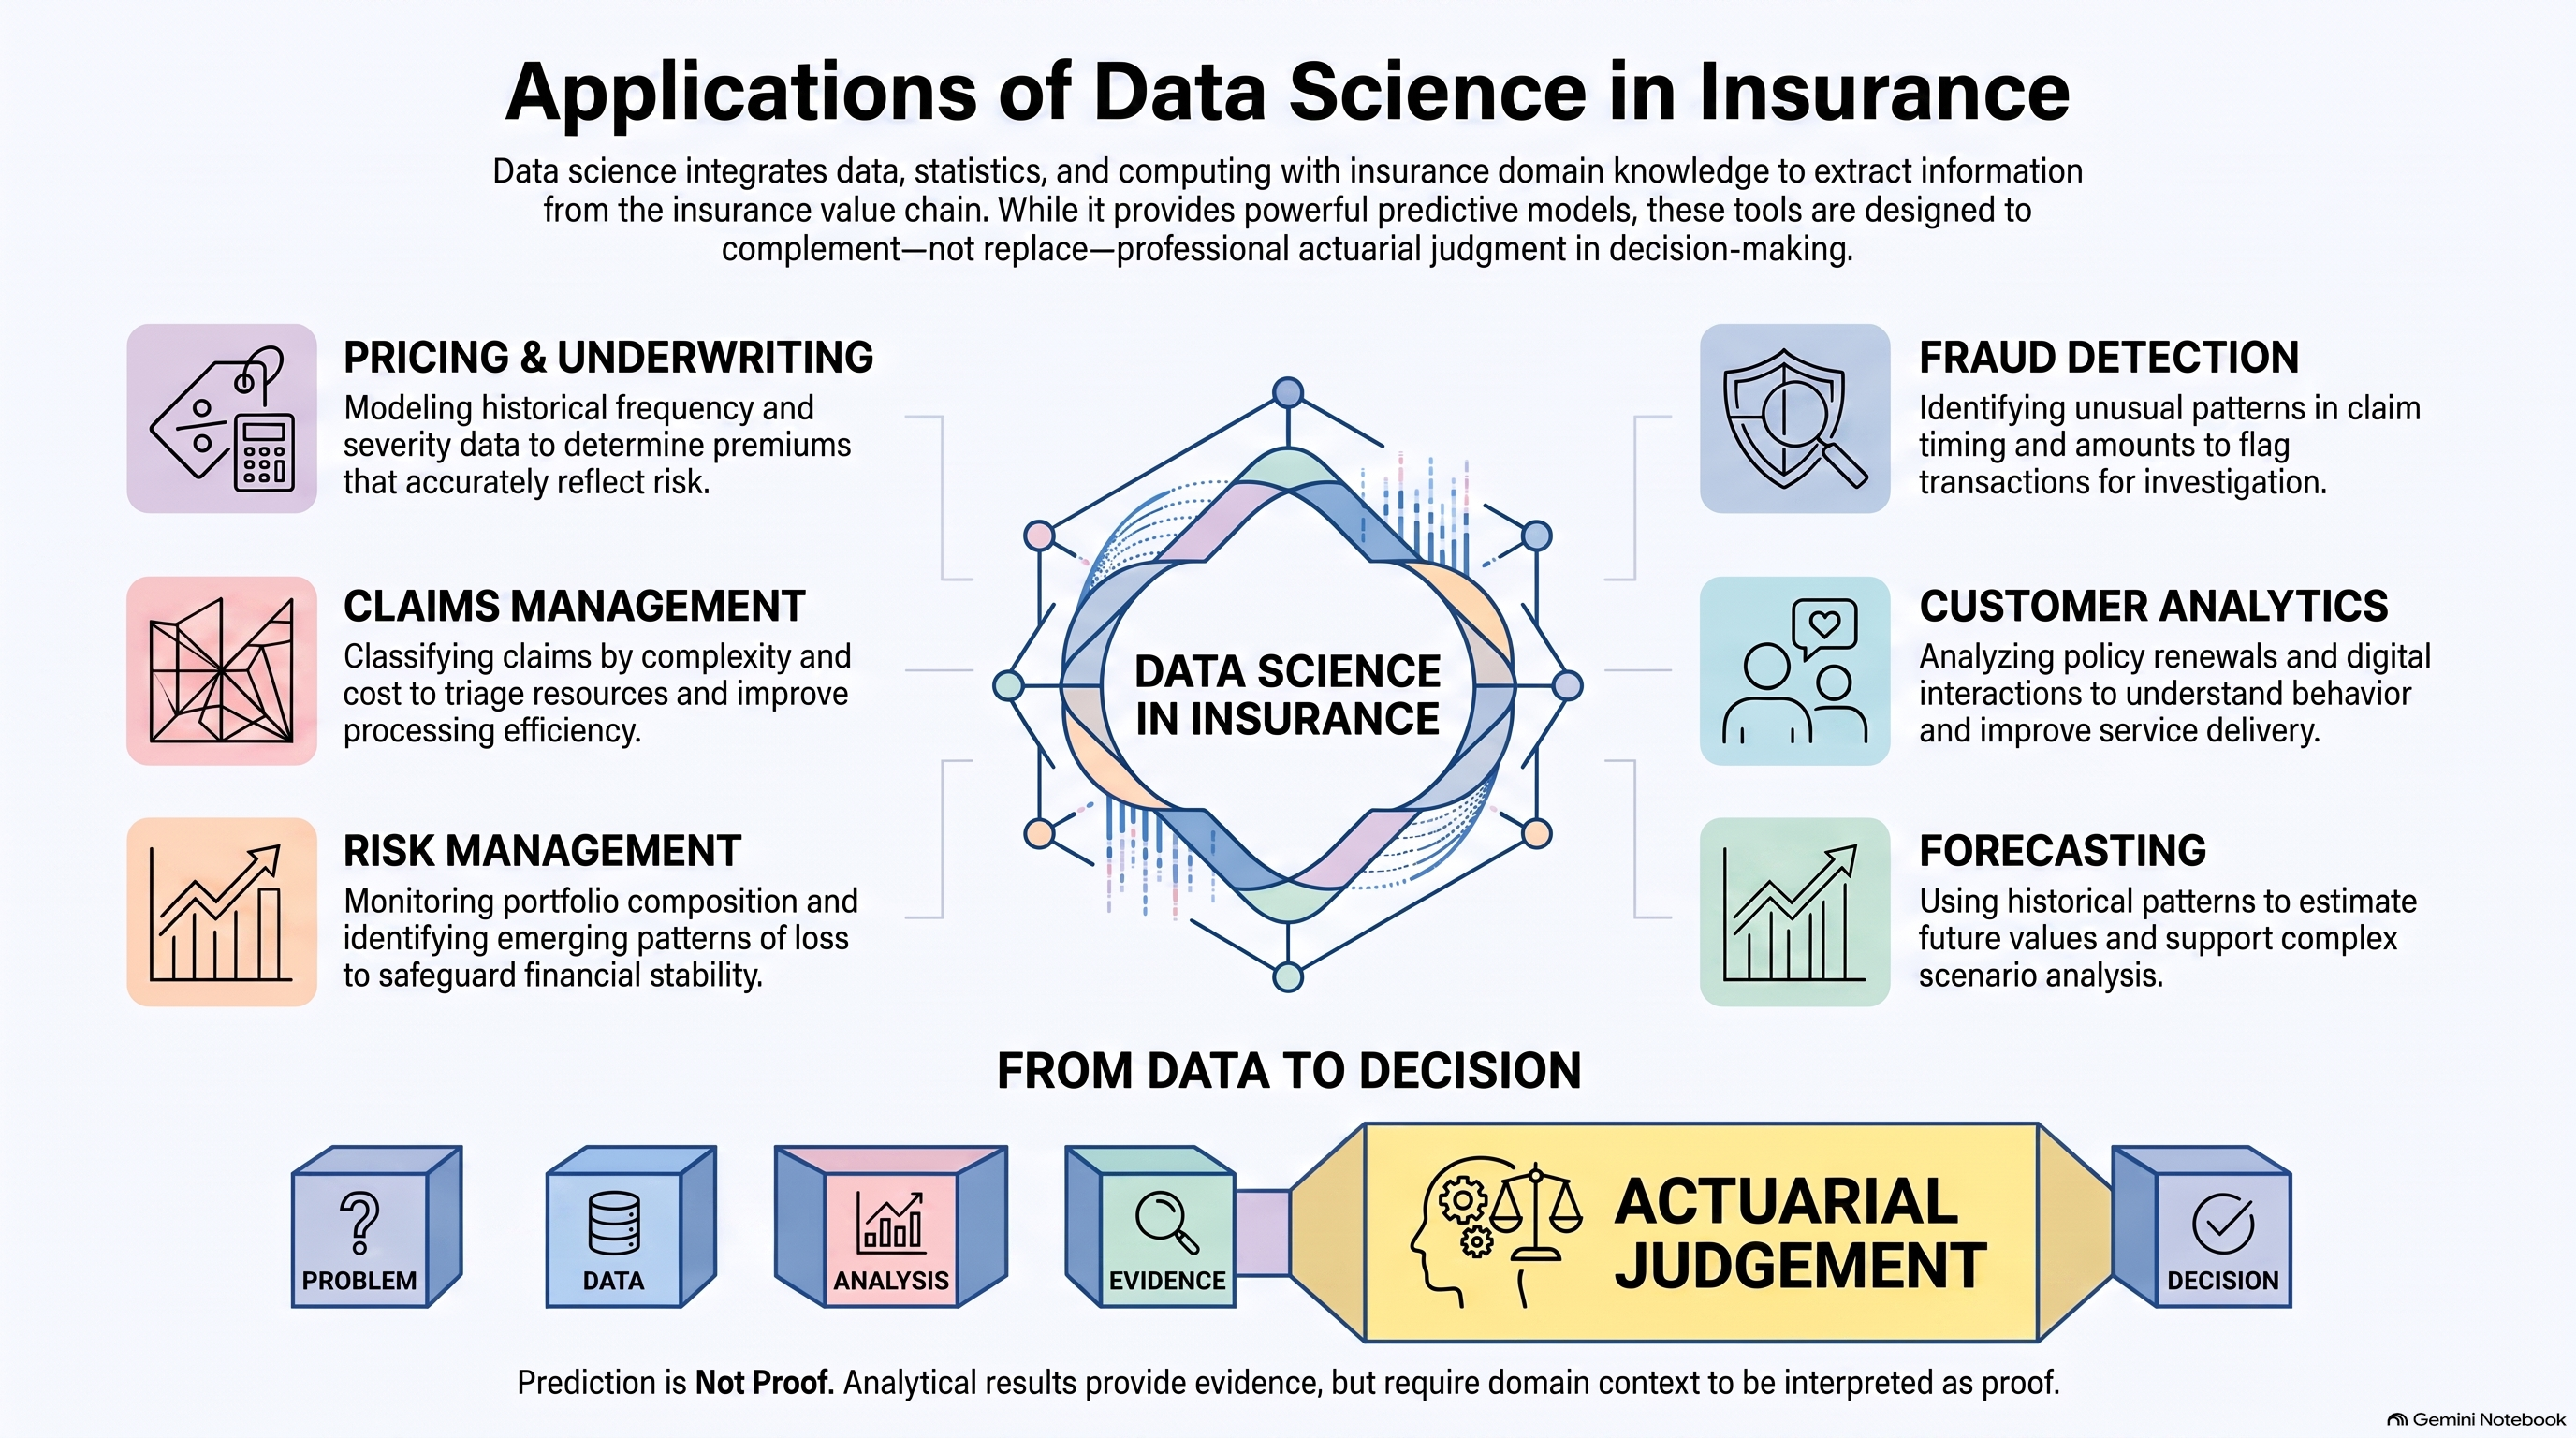
\includegraphics[width=0.78\linewidth,height=\textheight,keepaspectratio]{figures/Data_Science_in_Insurance_Applications.png}

}

\caption{\label{fig-insurance-apps-slides}Data Science Applications in
the Insurance Industry}

\end{figure}%

The methods may differ across applications, but the underlying
data-science principles remain similar.
\end{frame}

\begin{frame}{Common Applications}
\protect\phantomsection\label{common-applications}
Major applications include:

\begin{enumerate}
\tightlist
\item
  \textbf{Pricing and underwriting}
\item
  \textbf{Claims management}
\item
  \textbf{Fraud detection}
\item
  \textbf{Customer analytics}
\item
  \textbf{Risk management and forecasting}
\end{enumerate}

Each application begins with an insurance problem and uses relevant data
to support a decision.
\end{frame}

\begin{frame}{Pricing and Underwriting}
\protect\phantomsection\label{pricing-and-underwriting}
Pricing is one of the main applications of data science in insurance.

Insurers need to estimate the expected cost of claims and determine
premiums that appropriately reflect the risks being insured.

Historical policy and claims data can be used to investigate how
outcomes vary with:

\begin{itemize}
\tightlist
\item
  age;
\item
  geographical area;
\item
  vehicle characteristics;
\item
  coverage; and
\item
  other risk factors.
\end{itemize}
\end{frame}

\begin{frame}{Example: Motor Insurance Pricing}
\protect\phantomsection\label{example-motor-insurance-pricing}
Suppose an insurer wants to investigate whether claim frequency varies
with policyholder age.

Historical data can be used to:

\begin{enumerate}
\tightlist
\item
  measure claim experience;
\item
  explore differences between age groups;
\item
  identify relevant risk characteristics; and
\item
  develop a statistical model.
\end{enumerate}

The model can then estimate expected claim frequency for different
combinations of risk characteristics.
\end{frame}

\begin{frame}{Frequency and Severity in Pricing}
\protect\phantomsection\label{frequency-and-severity-in-pricing}
A simple representation of expected loss is

\[
\text{Expected loss}
\approx
\text{Expected frequency}
\times
\text{Expected severity}.
\]

Data science can support both components.

Historical data can be used to model:

\begin{itemize}
\tightlist
\item
  the number of claims; and
\item
  the amount of individual claims.
\end{itemize}

Other variables can then be used to explain differences in risk.
\end{frame}

\begin{frame}{Data Science Does Not Replace Actuarial Pricing}
\protect\phantomsection\label{data-science-does-not-replace-actuarial-pricing}
A predictive model provides estimates based on data and modelling
assumptions.

A pricing decision may also require consideration of:

\begin{itemize}
\tightlist
\item
  expenses;
\item
  capital;
\item
  reinsurance;
\item
  regulatory requirements;
\item
  market conditions; and
\item
  professional judgement.
\end{itemize}

\begin{tcolorbox}[enhanced jigsaw, arc=.35mm, bottomrule=.15mm, bottomtitle=1mm, breakable, colback=white, colbacktitle=quarto-callout-note-color!10!white, colframe=quarto-callout-note-color-frame, coltitle=black, left=2mm, leftrule=.75mm, opacityback=0, opacitybacktitle=0.6, rightrule=.15mm, title=\textcolor{quarto-callout-note-color}{\faInfo}\hspace{0.5em}{Key idea}, titlerule=0mm, toprule=.15mm, toptitle=1mm]

\textbf{A predictive model is one input into an actuarial pricing
decision.}

It does not determine the final premium by itself.

\end{tcolorbox}
\end{frame}

\begin{frame}{Claims Management}
\protect\phantomsection\label{claims-management}
Claims generate a substantial amount of information that can be
analysed.

Data science can support:

\begin{itemize}
\tightlist
\item
  understanding claim patterns;
\item
  estimating expected claim costs;
\item
  predicting claims outcomes; and
\item
  claims triage.
\end{itemize}

For example, claims may be classified according to:

\begin{itemize}
\tightlist
\item
  type;
\item
  estimated cost;
\item
  complexity; or
\item
  likelihood of requiring further investigation.
\end{itemize}
\end{frame}

\begin{frame}{Using Data to Prioritise Claims}
\protect\phantomsection\label{using-data-to-prioritise-claims}
Predictive models can help identify claims that are likely to:

\begin{itemize}
\tightlist
\item
  become large; or
\item
  require additional attention.
\end{itemize}

This can help claims staff allocate resources more effectively.

The objective is not necessarily to automate the entire claims process.

Analytical results can instead provide additional information to claims
professionals when making decisions.
\end{frame}

\begin{frame}{Monitoring Claims Experience}
\protect\phantomsection\label{monitoring-claims-experience}
Data can also be used to monitor the development of claims over time.

For example, observed claim experience can be compared with:

\begin{itemize}
\tightlist
\item
  previous experience; or
\item
  expected outcomes.
\end{itemize}

Differences may provide information for claims management and portfolio
monitoring.
\end{frame}

\begin{frame}{Fraud Detection}
\protect\phantomsection\label{fraud-detection}
Insurance fraud can result in financial losses and affect the overall
cost of insurance.

Data science can help identify claims or transactions with unusual
characteristics.

Relevant information may include:

\begin{itemize}
\tightlist
\item
  policy characteristics;
\item
  claim characteristics;
\item
  claim timing;
\item
  claim amounts; and
\item
  previous claims.
\end{itemize}
\end{frame}

\begin{frame}{Identifying Unusual Claims}
\protect\phantomsection\label{identifying-unusual-claims}
Statistical or machine-learning methods can identify patterns associated
with claims that require further investigation.

The model may identify a claim as unusual.

However:

\[
\boxed{
\text{Unusual pattern}
\neq
\text{Proof of fraud}
}
\]
\end{frame}

\begin{frame}{Prediction Is Not Proof}
\protect\phantomsection\label{prediction-is-not-proof}
A model can:

\begin{itemize}
\tightlist
\item
  identify unusual patterns;
\item
  estimate probabilities; or
\item
  rank cases according to predicted risk.
\end{itemize}

It does \textbf{not} automatically establish that a particular
policyholder has committed fraud.

\begin{tcolorbox}[enhanced jigsaw, arc=.35mm, bottomrule=.15mm, bottomtitle=1mm, breakable, colback=white, colbacktitle=quarto-callout-important-color!10!white, colframe=quarto-callout-important-color-frame, coltitle=black, left=2mm, leftrule=.75mm, opacityback=0, opacitybacktitle=0.6, rightrule=.15mm, title=\textcolor{quarto-callout-important-color}{\faExclamation}\hspace{0.5em}{Prediction is not proof}, titlerule=0mm, toprule=.15mm, toptitle=1mm]

A data-science model can identify patterns or assign a probability to an
outcome.

The result should not automatically be interpreted as proof that fraud
has occurred.

Further investigation and appropriate professional procedures are
required.

\end{tcolorbox}
\end{frame}

\begin{frame}{Customer Analytics}
\protect\phantomsection\label{customer-analytics}
Data science can also be used to understand customer behaviour and
interactions with insurers.

Examples include analysing:

\begin{itemize}
\tightlist
\item
  policy renewals;
\item
  cancellations and lapses;
\item
  customer enquiries;
\item
  product preferences; and
\item
  interactions with digital services.
\end{itemize}
\end{frame}

\begin{frame}{Example: Policy Lapse}
\protect\phantomsection\label{example-policy-lapse}
Suppose an insurer wants to identify policies with a high probability of
not being renewed.

Historical policy data can be used to:

\begin{enumerate}
\tightlist
\item
  identify previous renewal patterns;
\item
  develop a predictive model;
\item
  identify characteristics associated with higher lapse rates; and
\item
  support decisions about customer communication.
\end{enumerate}

The results may inform:

\begin{itemize}
\tightlist
\item
  customer communication;
\item
  product design; and
\item
  service delivery.
\end{itemize}
\end{frame}

\begin{frame}{Risk Management and Forecasting}
\protect\phantomsection\label{risk-management-and-forecasting}
Data science can support broader risk-management and forecasting
activities.

Insurers need to monitor changes in their portfolios and anticipate
future outcomes.

Historical data can be used to identify:

\begin{itemize}
\tightlist
\item
  trends;
\item
  changes in risk characteristics; and
\item
  unusual patterns.
\end{itemize}
\end{frame}

\begin{frame}{Examples of Forecasting Applications}
\protect\phantomsection\label{examples-of-forecasting-applications}
Examples include:

\begin{itemize}
\tightlist
\item
  forecasting claim volumes;
\item
  monitoring changes in claim severity;
\item
  analysing portfolio composition;
\item
  identifying emerging patterns of loss; and
\item
  supporting scenario analysis.
\end{itemize}

Forecasting methods use historical patterns and other relevant
information to estimate future outcomes.
\end{frame}

\begin{frame}{Forecasts Are Uncertain}
\protect\phantomsection\label{forecasts-are-uncertain}
A forecast is subject to uncertainty.

Future insurance experience may differ from historical experience
because of changes in:

\begin{itemize}
\tightlist
\item
  economic conditions;
\item
  technology;
\item
  regulation;
\item
  customer behaviour; or
\item
  the underlying risk environment.
\end{itemize}

Therefore,

\[
\boxed{
\text{Historical pattern}
\not\Rightarrow
\text{Certain future outcome}
}
\]

Forecasting requires both statistical analysis and careful
interpretation.
\end{frame}

\begin{frame}{From Data to Insurance Decisions}
\protect\phantomsection\label{from-data-to-insurance-decisions}
The applications above use different methods, but they share a common
process:

\[
\boxed{
\text{Problem}
\;\rightarrow\;
\text{Data}
\;\rightarrow\;
\text{Model}
\;\rightarrow\;
\text{Evidence}
\;\rightarrow\;
\text{Judgement}
\;\rightarrow\;
\text{Decision}
}
\]

This is the same data-science life cycle introduced earlier.
\end{frame}

\subsection{Part VII --- Putting the Ideas
Together}\label{part-vii-putting-the-ideas-together}

\begin{frame}{Data Science Across Insurance}
\protect\phantomsection\label{data-science-across-insurance}
Data science is not a single insurance technique.

It is a collection of methods that can support different types of
insurance decisions.

The same general process applies to:

\begin{itemize}
\tightlist
\item
  pricing;
\item
  claims management;
\item
  fraud detection;
\item
  customer analytics; and
\item
  risk management.
\end{itemize}
\end{frame}

\begin{frame}{One Framework, Many Applications}
\protect\phantomsection\label{one-framework-many-applications}
{\def\LTcaptype{none} % do not increment counter
\begin{longtable}[]{@{}lll@{}}
\toprule\noalign{}
Application & Main question & Example output \\
\midrule\noalign{}
\endhead
Pricing & How does expected loss vary with risk? & Risk estimate \\
Claims & Which claims require attention? & Claim classification \\
Fraud & Which cases are unusual? & Investigation priority \\
Customer analytics & Which policies may lapse? & Lapse probability \\
Risk management & What may happen in the future? & Forecast \\
\bottomrule\noalign{}
\end{longtable}
}

The analytical methods differ, but the underlying process is similar.
\end{frame}

\begin{frame}{The Common Process}
\protect\phantomsection\label{the-common-process}
\[
\boxed{
\text{Question}
\rightarrow
\text{Data}
\rightarrow
\text{Analysis}
\rightarrow
\text{Evidence}
\rightarrow
\text{Decision}
}
\]

The process connects technical data analysis with the original insurance
problem.
\end{frame}

\begin{frame}{Data Science and Actuarial Judgement}
\protect\phantomsection\label{data-science-and-actuarial-judgement}
Data science provides methods for extracting information from data.

Actuarial knowledge provides the context needed to:

\begin{itemize}
\tightlist
\item
  formulate the insurance problem;
\item
  understand the data;
\item
  assess assumptions;
\item
  interpret results; and
\item
  consider the consequences of a decision.
\end{itemize}

Therefore,

\[
\boxed{
\text{Data science}
+
\text{Actuarial knowledge}
\rightarrow
\text{Better-informed insurance decisions}
}
\]
\end{frame}

\begin{frame}{Key Ideas from the Chapter}
\protect\phantomsection\label{key-ideas-from-the-chapter}
By the end of this chapter, you should be able to:

\begin{itemize}
\tightlist
\item
  explain why data science is relevant to insurance;
\item
  describe the four foundations of data science;
\item
  identify common sources and types of insurance data;
\item
  describe the data science life cycle;
\item
  explain the roles of different members of a data science team;
\item
  identify major applications of data science in insurance; and
\item
  explain how data-driven evidence is combined with actuarial judgement.
\end{itemize}
\end{frame}

\begin{frame}{The Big Picture}
\protect\phantomsection\label{the-big-picture}
The central idea of this chapter is:

\[
\boxed{
\begin{array}{c}
\text{Insurance problem}
\\[4pt]
\downarrow
\\[4pt]
\text{Relevant data}
\\[4pt]
\downarrow
\\[4pt]
\text{Data science life cycle}
\\[4pt]
\downarrow
\\[4pt]
\text{Evidence}
\\[4pt]
\downarrow
\\[4pt]
\text{Actuarial judgement}
\\[4pt]
\downarrow
\\[4pt]
\text{Insurance decision}
\end{array}
}
\]

Data science provides a framework for turning data into evidence.

Actuarial knowledge provides the context needed to interpret that
evidence and use it appropriately.
\end{frame}

\begin{frame}{Looking Ahead}
\protect\phantomsection\label{looking-ahead}
The next chapters will develop the tools needed to work through this
process.

We will move from the general framework introduced here to practical
methods for:

\begin{itemize}
\tightlist
\item
  working with data;
\item
  exploring and visualising data;
\item
  applying statistical methods; and
\item
  using computational tools for data analysis.
\end{itemize}

The objective is to connect these methods to actuarial and insurance
problems.
\end{frame}




\end{document}
